%%%%%%%%%%%%%%%%%%%%%%%%%%%%%%%%%%%%%%%%%%%%%%%%%%%%%%%%%%%%%%%%%%%%%%%%%%
%% This is a document template for an Otago thesis (Masters or PhD).
%% A skeleton chapter layout is also suggested.
%%
%% Look in the directory example_document for filled-out chapters
%% that show you how to do figures, bibliographies, and tables.
%%
%% Since this was written for Computer Science at Otago University,
%% Harvard (author, date) style citations are used.  Other students
%% should consult their advisors as to what style of citations to use.  
%%
%% Nathan Rountree 9/2/98
%%
%%%%%%%%%%%%%%%%%%%%%%%%%%%%%%%%%%%%%%%%%%%%%%%%%%%%%%%%%%%%%%%%%%%%%%%%%%%

%%
%% In the style of a technical report, in 12pt and one sided.
%% Start chapters on right hand side pages only.
%%
\documentclass[12pt]{report}    
%%\documentclass[12pt,twoside,openright]{report} %% Use this for twosided.

%%
%% Load packages.
%%

\usepackage[phd]{otagothesis}     %% Use Otago page layout
\usepackage{graphicx}
\usepackage{url}
\renewcommand{\abstractname}{\vspace{-\baselineskip}}
\usepackage{cite}
%\usepackage[longnamesfirst,round]{natbib} %% Use Natural Sciences bibliography
\usepackage[authoryear, round]{natbib} %% Use Natural Sciences bibliography
%\usepackage[numbers]{natbib}

%\usepackage[longnamesfirst, round]{natbib}

%\usepackage[table]{xcolor}
%\usepackage{multirow}
%\usepackage{array}
%\usepackage{amstext}
%\usepackage{blindtext}

%\usepackage{textcomp}
\usepackage{caption}
\usepackage{subcaption}
%%\usepackage{times}              %% Times PostScript font. Don't use
				  %% if thesis contains lots of math.
\usepackage{algorithm}
%\usepackage{graphicx}             %% jpg, gif, tiff, and pdf graphics
\usepackage{moreverb}             %% Verbatim Code Listings
\usepackage{algorithmic}
\usepackage{framed}

\renewcommand{\algorithmicrequire}{\textbf{Input:}}
\renewcommand{\algorithmicensure}{\textbf{Output:}}
%%
%% Set title, author and date.
%%
\title{Indoor scene positioning for blind people using vision}
\author{Nabeel Younus Khan}
\date{30 June 2013}

%%
%% The library want to know all sorts of personal stuff!
%% Can be left out if you don't use the \frontstuff command
%%
\fullname{Nabeel Younus Khan}
\department{Department of Computer Science}
\dob{17 December 1982} %% date-of-birth
\address{85 Harrow Street, North Dunedin, NZ}

%%
%% Uncomment to just print up a few chapters.
%%
%%\includeonly{literature,conclusion}

%%
%% Go!
%%
%\usepackage {float}

\begin{document}
%%
%% Put in titlepage and contents, etc...
%%
\frontstuff

%%
%% Set to one-and-a-half line-spacing
%%
\linespread{1.3} \normalsize

%%
%% Include each chapter as a separate file.
%% These lines assume there are files called intro.tex, literature.tex etc.
%%

\chapter{Introduction}
\label{chap:intro}

Navigation systems assist the
process of localizing, planning and following a specific route 
where localization refers to identify one's position in space.
The location information is firstly used by the navigation 
system to identify the current position on the map and 
secondly to guide the movement from one point to the other. 
A precise localization is therefore 
very important and is required for an effective 
performance of a navigation system.
The navigation systems provide
assistance either to the visually impaired people 
(especially blind) or robots. Blind people or 
robots both have no perception about the 
environment surroundings and require step by step instructions 
to navigate in unfamiliar environments via 
voice messages or control signals. 

%Localization is the basic requirement to navigate in an environment. 
The localization is not a problem for humans 
without any visual impairment. 
They extract and use different pieces of information 
such as landmarks, sign boards, color cues, object etc 
from the current scene to recall and recognize the current 
place. But on the other hand, blind people
cannot use any visual clues for the localization. 
The blind person has only access to the sound information 
of the surroundings but that information is either 
not enough or totally missing. Therefore, blind 
people rely totally on near by people for the 
desired information. Blind people need the 
positioning information quite often 
for a rough guidance during navigation in 
in unfamiliar environments which highlights 
the importance of a robust localization.


The basic localization can be achieved without any special instruments 
e.g. sailors have been using astronomical objects 
for localization for a thousand years during sea travel. 
Many specialized tools were
developed for more accurate localization 
during the early centuries 
most notably the astrolabe, compass, sextant, 
marine chronometer etc.
The major advancements in this area are 
observed in the 20th century and different 
electronic tools have been invented.
In the 1920s, the localization based on radio signals from 
shore based transmitters was proposed 
which helped in further improving the sea based navigation . 
The first practical radar system was developed in 1935 
which was capable of determining the 
presence and range of an object, its position in space,
its size and shape etc. It was used for marine, controlling air traffic, 
detecting weather patterns and tracking spacecraft.
In the late 1960s, the United States 
Department of Defense began developing a 
satellite based localization system for military purposes
which eventually led to the Global Positioning System (GPS) in 1978 (\cite{pace95}). 
This space based radio navigation system
provided accurate positioning to within about 30 feet 
as well as velocity and time worldwide in any weather conditions.
The modern GPS systems can provide accuracy up 
to 3 meters. 


GPS is the most popular system to find the location
and the position of the objects for navigation systems. 
It receives signals from multiple satellites 
and determines the physical location through a 
triangulation process. 
GPS work extremely well in outdoor 
but GPS satellites are often 
occluded by buildings or trees in urban environments. 
Therefore many systems use GPS information along with 
other sensors such as vision(~\cite{agrawal06, leung08}), 
geographical information system (~\cite{ boonifait08}), 
inertial measurement units (~\cite{georgy11}) etc 
for better performance during urban navigation. 


GPS is an outdoor positioning system 
and does not work in indoor because GPS 
signals cannot penetrate in the buildings. 
However high sensitivity GPS can provide indoor 
positioning but signals are heavily attenuated 
and reflected by the building materials making it 
highly unreliable. It's is also hard to extract reliable 
high level details such as floor level information 
etc from GPS signals. 
The indoor localization without GPS is still an open 
and universal research problem. 
The cameras have proven to be 
good sensors for indoor positioning 
in terms of cost and reliability (~\cite{davidf07, hongwen09}). 
The localization systems based on vision attempt 
to match the captured image of the current scene 
with a labeled database 
of trained images to identify the current location. 
There are two main problems with most of the existing 
indoor vision based solutions: (1) few indoor places are used 
for experiments, and (2) focus is kept on non-office buildings.
The scene localization becomes quite 
challenging in office indoor buildings where 
different places look much similar as shown in 
Figure \ref{fig:sampleindoor}. 

\begin{figure}[h!]
\centering
        \begin{subfigure}[b]{0.40\textwidth}
                \centering
                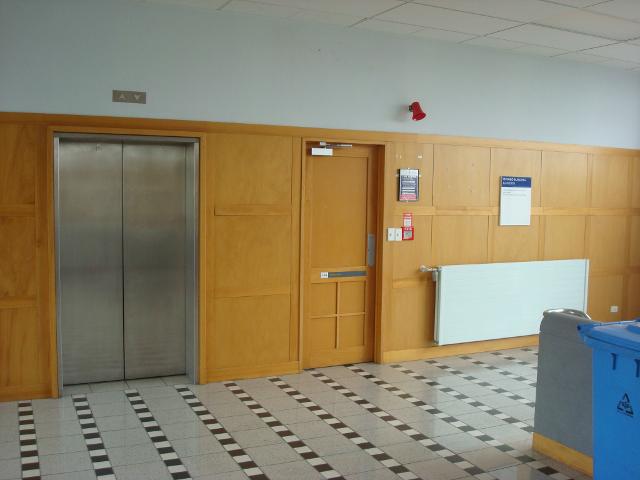
\includegraphics[width=\textwidth]{images/indoor.png}
                \caption{Central hall of 3rd floor.}
                \label{fig:sifta}
        \end{subfigure}
        \begin{subfigure}[b]{0.40\textwidth}
                \centering
                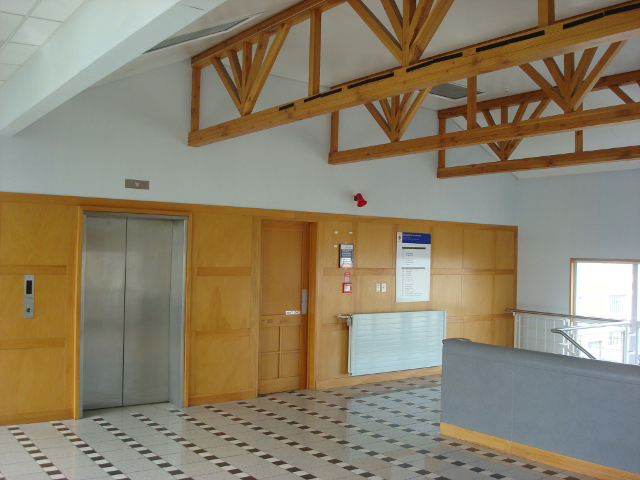
\includegraphics[width=\textwidth]{images/indoor1.png}
                \caption{Central hall of second floor.}
                \label{fig:siftb}
        \end{subfigure}
      \caption{Images of two locations with in the office building with huge similarities.}
 \label{fig:sampleindoor} 
\end{figure}


In order to address the mentioned limitations,
we have proposed an "Indoor Positioning System (iPoS)" which is currently 
based on a client server model and targets the blind users. 
The smartphone application 
allows its user to take a picture of the indoor scene, sends 
it to the server to find the best match and then 
generates a voice message on the smartphone 
to indicate the current location. 
The algorithms which enable iPoS to operate robustly include 
firstly, a proposed visual Bag of Words (BoW) 
scheme for relevant image retrieval. 
Secondly a verification method to verify the location 
match followed by further validation if required.
We have tested our system
in large indoor environments and got good results. 
Our results show that single camera is 
a feasible sensor for indoor positioning 
in real time in challenging indoor environments.

%-------------------------------------------------------------------
\section{Motivation}
\label{sec:motivation}
There are about 11,500 people in New Zealand 
who are either blind or have a low vision (~\cite{rnzfb}).
By 2020, the population of blind people in New Zealand 
is estimated to rise up to 18,300. While population 
of blind people have risen to 39 million all over 
the world lately (~\cite{who12}).
Therefore, a cost effective solution 
is required for the blind people in coming years.

Indoor positioning systems based on non-vision 
sensors such as infrared light (~\cite{roy92}), 
ultrasonic (~\cite{ko08}), Wi-Fi (~\cite{paul08}) 
and Active-RFID (~\cite{ni04}) have been proposed. 
The indoor localisation system based on any sensor 
should at least meet some requirements: (1)
equipment cost should be less, 
(2) positioning accuracy should be high,  
(3) handling of multiuser should be there, 
and (4) easy to use for the blind people.
The performance comparison of different sensors 
keeping in mind the mentioned requirements 
in summarized in Table \ref{tab:tech} (~\cite{kawaji10}). 
The image processing or vision solutions based 
on a mobile camera seem to offer 
a cost effective solution with reasonable accuracy. 
Therefore, the main motivation our research work is to:

\emph{
\begin{quote}
come up with a robust localization system based solely on vision 
which is easy to use and can provide rough guidance 
to blind people during navigation 
in office and non-office buildings. 
\end{quote}
}
\begin{table}

\caption{Performance comparison of existing technologies}
\centering
\begin{tabular}{|c|c|c|}
\hline 
Technology & Positioning accuracy & Equipment cost\tabularnewline
\hline
\hline 
Infrared light  & 5-10m  & High \tabularnewline
\hline 
Ultrasonic  & 1-10cm  & High \tabularnewline
\hline 
RFID  & 5cm-5m  & High \tabularnewline
\hline 
Wi-Fi  & 2-100m  & Low-High \tabularnewline
\hline 
Audible sound  & 5-10m  & Middle \tabularnewline
\hline 
Mobile camera & 1-5m  & Low \tabularnewline
\hline
\end{tabular}
\label{tab:tech}
\end{table}




The other motivators for our work are:-

\begin{itemize}
\item Most vision based localization works 
focus  on outdoor environments. 

\item The literature shows not much work 
is done in large scale indoor environments 
using vision. Most works limit experiments 
to few indoor places. 

\item Localisation is often performed 
in context of non office buildings. The 
positioning becomes a challenge in office 
buildings where places are pretty similar. 
Therefore, a localisation system performance 
needs to be analysed in office environment.

\item Video stream is used as an input 
for the real time localization and mapping 
in many works (~\cite{gemeiner08}). 
This is not ideal for blind people
because video stream will drain the 
phone battery and will require 
often charging of the phone. This will 
only add more to the worries of 
blind people.

\item The localization module is often embedded 
in the navigation systems and is not available 
as a separate independent unit.
\end{itemize}



Blind people carry smart phones for making calls, 
reading emails etc and are familiar with most of 
the functionality. The majority of the smartphones 
has a reasonable camera and a 
smartphone application based on vision 
will be really handy 
for the blind people. Blind people can use the 
application when they feel they are lost 
while navigating in indoor buildings. 

%-------------------------------------------------------------------
\section{Challenges and contributions}
\label{sec:contributions}
Most of the successful scene recognition work is 
done in outdoor environments. 
Comparatively, less work is done for office indoor buildings.
It's quite hard to find a framework in which smartphone 
uses a single image of the current scene and 
performs a robust localization. Amongst, the challenges 
we faced were:-

\begin{itemize}

\item Identifying the reliable features
which are capable of good image matching 
with different transformations 
in any environment. 


\item People propose and use different techniques to verify 
the images retrieved from visual BoW but 
on different data sets. 
So there is no standard way for
images verification. 

\item The absence of office building data sets 
for the experimental purposes. 

\item Designing a user friendly interface 
for our smartphone application to 
ptovide maximum accessibility to the 
blind uers.


\item Understanding the camera model coordinate 
systems and transformations 
between 2D features (query image) 
and 3D models (points) for effective pose estimation.

\end{itemize}

We followed a bottom up approach. We first identified the 
best features to be used for image matching 
in our work. We then started with the 
image matching in outdoor environment 
followed by the experiments in our indoor data set. 
After a careful analysis, we proposed a 
robust image matching system which 
can localize the current scene. Finally, we 
developed the smartphone application to send 
the query pictures to our system (running on a 
server) and evaluated the localisation performance 
on real indoor data sets. 
Our main contributions are:-


\begin{itemize}
\item We propose a shorter version of scale invariant feature 
transform (SIFT) features (~\cite{khan12b}) 
for the image matching and compare it with other well known feature 
descriptors.

\item We evaluate the performance of our 
shorter SIFT features thoroughly against 
different image transformations (~\cite{khan11b}). 

\item We evaluate different ranking functions 
namely normalized term frequency ($ntf$), normalized term 
frequency inverse document frequency ($ntfidf$) and 
Okapi $BM25$ for the visual BoW for the analysis. 

\item We compare soft and hard 
assignments schemes  in visual BoW 
for the indoor environment (~\cite{khan11a}). 


\item We propose a visual BoW based on 
a voting module and a verification method. Voting module 
is not only efficient but also effective.


\item We compare different verification methods 
with our proposed homography method for the analysis (~\cite{khan11a}).
Our proposed homography verification method 
gives comparable performance to the fundamental 
matrix based verification and is also efficient. 

\item We propose a track based approach to 
effectively reduce the features from large scale data sets 
up to a 50\%~\cite{khan12c}.


\item We develop a working android application (~\cite{khan12a}). 
The application is refined over time 
in functionality and thoroughly tested on various 
indoor data sets. The current application offers the 
simplest interface which is suitable for blind users (~\cite{khan12b}). 


\item We compare the localisaiton performance 
based on pose estimation and 2D image matching 
with different mobile devices for analysis.
We also propose a hybrid algorithm 
for an effective indoor image matching 
with almost zero wrong matches. 

\item We develop five indoor data sets which 
can be used as a standard to test the classification 
performance in indoor. 
\end{itemize}


%-------------------------------------------------------------------
\section{Application}
\label{sec:applications}

Our system is intended to assist the blind people 
whilst they navigate in indoor buildings. However, 
it is also applicable to other users:-

\begin{enumerate}
\item \textbf{Prospective Students :}
It's hard to figure out the different places 
in the campus in the beginning. Our application 
can offer a natural way of learning information about
the campus by taking pictures and getting pop up 
text messages. The new students can utilize 
this application to get familiar 
with the campus environment. 

\item \textbf{Large malls: } 
It's easy to get lost in 
large shopping malls. This application could help 
shoppers to find where they are and where they want to go.


\item \textbf{Tourists: } 
Each city has a history reflected by the historic landmarks 
(e.g. buildings, statues, historic trees etc).
Our application can serve a guide for tourists, giving 
information about the captured landmark images 
from the smartphone therefore promoting the tourism.

\end{enumerate}


%---------------------------------------------------------------------
\section{Limit of scope}
\label{sec:limitofscope}
In simple scenario, the system takes the 
picture of the current scene and identifies the 
current location. In real time, there are different 
factors which can affect the performance of 
such system. It's is not possible to address all 
challenges in a single PhD project. The limitations of our work 
are:-

\begin{enumerate}
\item The initial target of our work 
was a complete navigation system for 
blind people but  we ended up with localization
due to time constraint. We also did not 
get time to integrate our localisation 
module with any existing navigation system for further 
analysis. 

\item We have not tested our system with blind 
users so far. However, the application may need to 
be voice powered (to launch/ close the application) 
to make it more accessible.

\item We use a non- incremental approach 
and the mapped images of the building are not 
updated whilst application performs localisaiton. 
The system does well with smaller changes with in the indoor 
places as shown in Figure \ref{fig:changes}. 
The maps will need updation 
if major changes happen in 
indoor places. This motivates the use 
of incremental approach to update the trained 
images during navigation (~\cite{angeli08}).
 
\begin{figure}[h!]
\centering
        \begin{subfigure}[b]{0.40\textwidth}
                \centering
                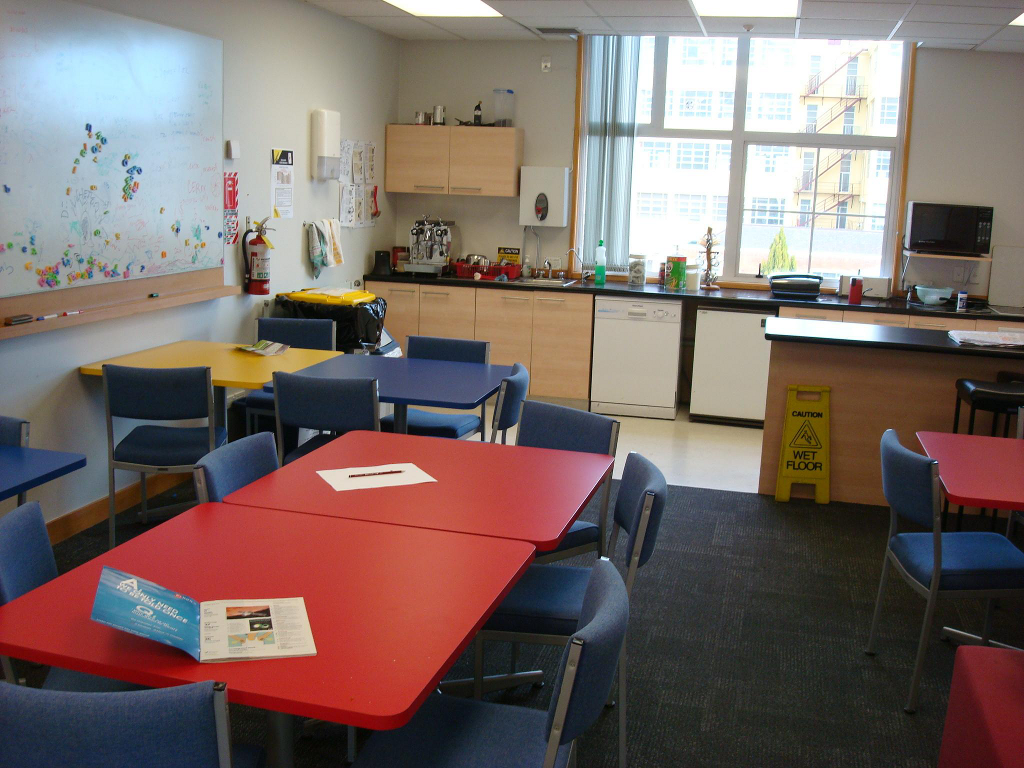
\includegraphics[width=\textwidth]{images/cr_1.png}
                \caption{Trained Image.}
        \end{subfigure}
        \begin{subfigure}[b]{0.40\textwidth}
                \centering
                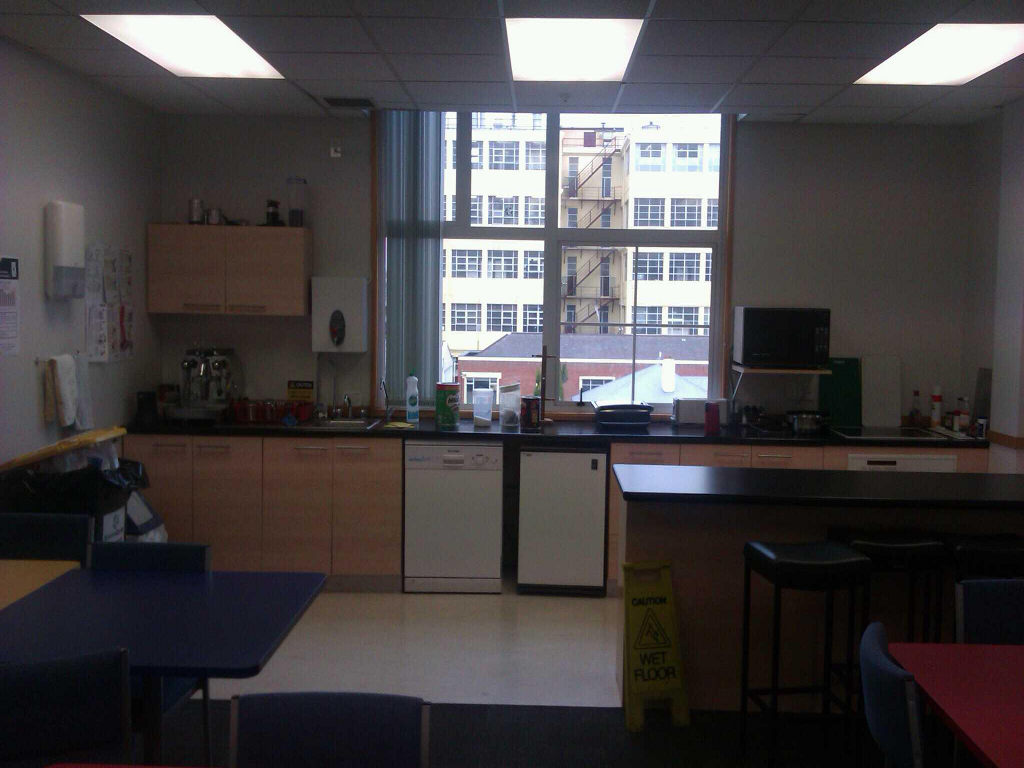
\includegraphics[width=\textwidth]{images/cr_2.png}
                \caption{Query Image.}
        \end{subfigure}
      \caption{Images of the same locations taken after some time.}
 \label{fig:changes} 
\end{figure}


\item Our system works well with a couple of people in the scene 
as shown in Figure \ref{fig:crowd}. The system capability to 
handle more people or crowd is not 
tested and is not the focus of our work.
 
\begin{figure}[h!]
	\centering
                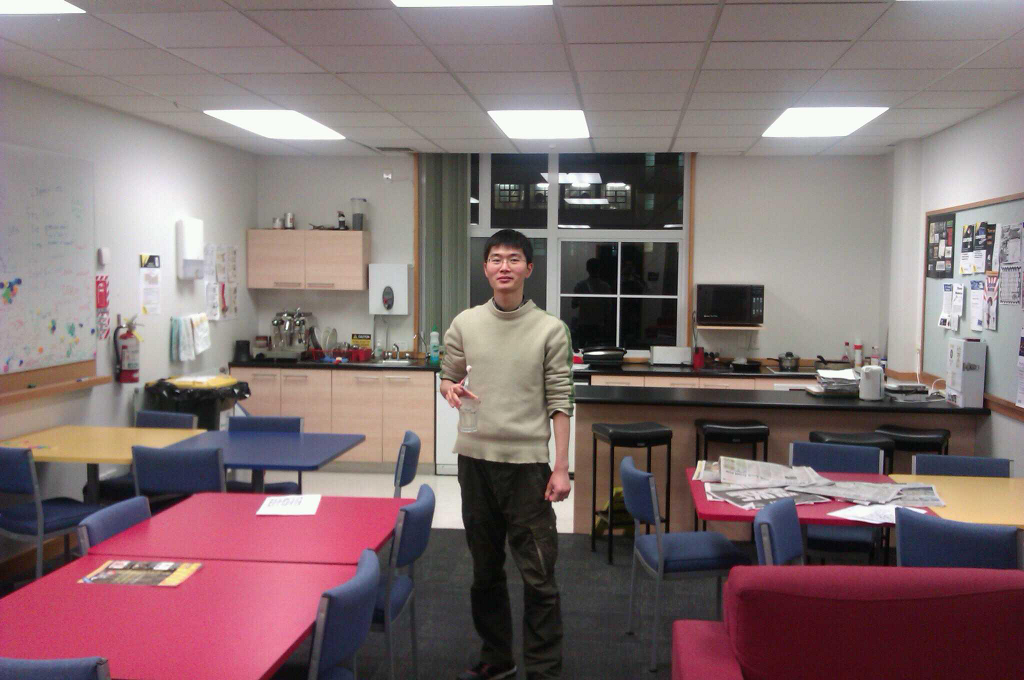
\includegraphics[width=0.4\textwidth]{images/crowd.png}
	      \caption{Query image taken at night.}
 \label{fig:crowd} 
\end{figure}


\item Our vision based localization system 
currently runs on the server. The smartphone 
application is just an interface for sending pictures 
and getting location information. We use 
this configuration for simplicity but 
whole system can be deployed on the smartphone. 



\item The mapped images of the building 
intended for navigation must be 
be labeled. We have developed "Map builder" 
module which needs an excel file filled from the user 
to generate the labels. The automatic labeling 
can also be done by using scene semantics 
or by image classification (~\cite{rasiwasia08, ranga10})
and is not the focus of our work.

\end{enumerate}

%----------------------------------------------------------
\section{Thesis Layout}
\label{sec:overview}

This thesis describes the development of iPoS. 
To achieve this, the used algorithms and corresponding evaluations 
on data sets are discussed in the chapters one by one. 
This thesis consists of nine chapters and details are 
as follows:-

\begin{enumerate}
\item \textbf{Chapter 2} gives an overview about 
navigation system requirements in context 
of blind users and presents some navigation 
tools which are in use of blind people.

\item \textbf{Chapter 3} presents research works 
which perform vision based indoor navigaiton 
and can guide the blind people. The localisation 
importance in visual navigation is further discussed followed 
by overview of some techniques used for indoor and 
outdoor scene recognition. 

\item \textbf{Chapter 4} states all data sets 
and metrics used in this thesis for performance 
evaluation. 

\item \textbf{Chapter 5} proposes a shorter versions of SIFT 
feature descriptor and compares it 
with different feature descriptors 
for general image matching on different data sets.

 \item \textbf{Chapter 6} proposes a visual Bag of Words (BoW) 
approach based on the shorter features proposed 
in Chapter 5. The proposed system is compared with 
a normal system with different configurations for 
performance analysis.

\item \textbf{Chapter 7} is a comparison 
of different verification methods 
which can be used with our proposed BoW presented 
in Chapter 6.

\item \textbf{Chapter 8} presents ways to reduce the 
features proposed in Chapter 4. The target 
was to use reduced features with proposed BoW 
for more robust image matching.

\item \textbf{Chapter 9} is evaluation of image localisation 
using pose estimation and simple 2D image matching 
with different mobile devices for the analysis. 

\item \textbf{Chapter 10} presents the framework 
used by us for the smartphone application. 
The system performance in real time data sets 
are reported in this chapter.

\item \textbf{Chapter 11} contains the final remarks 
and suggestions for possible future research work. 

\end{enumerate}

%----------------------------------------------------------
\section{Publications}
\label{sec:publicatios}

\begin{enumerate}
\item (~\cite{khan11a}) Proceedings of Image and Vision Computing New Zealand. 
This paper presents a proposed visual BoW 
based on voting scheme and homography method for a 
robust image matching.

\item (~\cite{khan11b})  Proceedings of International 
Conference on Digital Image Computing: 
Techniques and Applications (Australia). This paper discusses the proposed 
shorter version of SIFT features and compare it with SURF.

\item (~\cite{khan12a}) Proceedings of International 
Conference of the NZ Chapter of the 
ACM's Special Interest Group on Human-Computer Interaction. 
We discuss the first prototype of our smart phone application 
and reported the preliminary results. 

\item (~\cite{khan12b}) Proceedings of 14th International 
ACM SIGACCESS conference on Computers and Accessibility (USA).
We present the final prototype of our system 
and test it on larger images. 


\item  (~\cite{khan12c}) 
Proceedings of Image and Vision Computing New Zealand.
We propose the method to reduce the features from 
trained images by more than 50\% and compare 
our reduced features against well known descriptors.

\end{enumerate}
\subsection{APPSTAR Competition}
APPSTAR was a competition run by Otago Innovation Ltd, Otago University in 
2012. The competition asked the University of Otago’s academic and research 
staff and students all over the New Zealand 
to put forward an idea for a mobile or web Application. 
The competition received an incredible 108 entries and 
5 ideas were selected by a panel of Judges.
Our application in collaboration with William Levack 
'Living it up/iPos" was one of the top 5 finalists in the competition. 
The basic theme of 'Living it up/iPos" was 
to help people with memory loss to know exactly 
where they are in their house and then 
guide them to perform daily life time activities. 
For example if someone is in the kitchen 
then he/she can be prompted with a 
list of things to do such as make a breakfast, 
cooking tips etc.
 


%
\chapter{Navigation tools}
\label{chap:navtools}


This chapter discusses the requirements 
of a navigation system for a blind person 
in context of indoor and outdoor navigation. 
The popular navigation tools in use of
blind people are reviewed followed by 
some research projects which assist the 
navigation process.

%important presents reuiremneprovides an overview of some mobility 
%tools which assist the blind people during navigation. 
%The indoor navigation based on different 
%technologies such as WIFI, laser scanner etc is discussed. 
%Understanding the characteristics 
%and limitations of technologies is important to identify the 
%requirement of a vision based indoor navigation 
%system. Finally, the chapter highlights some of 
%the image based localisation works done in 
%indoor and outdoor environments. 

%------------------------------------------------------
\section{Navigation system requirements}
\label{sec:nsr}

Blind people need different functionalities from 
a navigation system. They make choices when it comes to travel and 
use different navigation tools depending upon their 
preferences.The navigation tools help the 
blind people to move safely in an environment. 
Different navigation tools are designed 
which address blind people requirements 
during the navigation. It is important to have a 
good understanding about these requirements 
before designing any navigation tool. 
Therefore, we began our research by conducting interviews 
with blind people. The interviews took place 
in Disability Information and Support Center, Otago 
University\footnote{\url{http://www.otago.ac.nz/disabilities/}}. 
The main purpose of the interview was the 
 requirement analysis i.e. figure out the 
functionalities, a blind person expects  from 
a navigation system. The requirements of a blind 
person from a navigation system 
are summarized as follows (~\citet{interview10}): 

\begin{itemize}
\item \textbf{Pedestrian Crossing:} 
The navigation system should guide the blind person
to remain in the center and to move in the right direction 
while on the pedestrian crossing. The crossing distance,
intersection street name, traffic rules etc information 
should also be communicated to increase the surroundings 
perception.

\item \textbf{Curbs Detection:}
The possible curbs or holes in the path 
should be detected and blind user should be alerted 
so that  precautionary steps can be taken 
to ensure the safety.  

\item \textbf{Sign boards:}
The system should recognize the places 
or landmarks  from sign boards. The location 
details along with the distance 
information to that landmark 
should be communicated to the user.

\item \textbf{Temporary Hazards:}
The temporary hazard signs such 
as wet floor signs, warning signs 
on a construction site etc must be detected 
and corresponding information 
should be communicated to the 
blind user. 

\item \textbf{Key destinations:}
The blind user should be guided to 
important city destinations such as hospitals, 
supermarkets, bus stops, airport etc.

\item \textbf{Speech accent:}
Navigation systems often use voice 
to communicate with its user but .
accent of the speech is sometimes 
not easy to understand. Therefore, a Braille display 
should also be available along 
with the system for further convenience.   

Braille displays are un-electro mechanical devices 
for displaying braille characters usually by means of 
raising dots through holes in a flat surface (~\citet{braille12}). 
Blind users use it to read text output.

\item \textbf{Indoor Localisation:}
Blind people want to know about 
their current indoor location in unfamiliar 
buildings and feel lost in the absence of such information. 
Therefore, a system with such functionality 
is required by the blind people. 

\item \textbf{Obstacle avoidance:}
The system should detect and alert user about 
the possible obstacles in the path to avoid the collision. 

\item \textbf{Toilets:}
The system should be able to classify the male 
and female toilets in buildings. 

\item \textbf{Scene description:}
Some sort of room description such as power socket location, 
exit doors information (opening inside/outside), 
wireless access points etc should be conveyed to the blind user. 
The location of power sockets is especially very 
important because blind people need to charge 
the carrying electronic devices. 

\item \textbf{Stairs:}
Blind people prefer lifts and the system 
should guide the blind users towards the lift. 
However, use of stairs should also be incorporated 
to deal with the emergency situations. 

\item \textbf{Guidance in the corridors:}
The system should indicate the steps 
information after which the turns are coming 
in the corridors of indoor buildings. 

\end{itemize}

Above, we have discussed the desired requirements from 
a navigation system for blind people. We realized from 
the interview that \emph{indoor localisation is one 
of the important requirement for blind people 
as they often visit unfamiliar buildings 
and have to rely on the near by people 
for the guidance.} 

It is quite hard to address all 
requirements in a single research work. 
However, these problems are addressed separately in 
different research works. Few vision based research works 
addressing the mentioned requirements are mentioned below:-

\begin{itemize}
\item (~\citet{coughlan07}) developed a 
navigation tool based on vision algorithm 
to detect the curbs and holes 
for blind wheelchair users. 
The disparity map is retrieved from stereo images 
followed by the generation of an edge map. 
On edge map, each pixel is checked for 
an appropriate depth leading to detection 
of possible curbs or holes and user is
alerted.

\item (~\citet{beno10}) presented a visual saliency 
based assistance system to point 
out areas of interest in a scene that 
present either particular interest or 
potential threat . 
The areas of interest refer to those 
objects that attract the visual attention 
of a human being. 

The system makes uses of a stereoscopic camera, 
a laptop and standard  headphones. 
The user first defines an objective such as 
find an object, find a door etc. Depending upon 
the objective, system computes the 
specific feature maps (colors, orientations, 
edges etc) and corresponding 
Conspicuity maps which lead to focuses 
of attention (FoA).  A conspicuity map 
contains information about regions of an 
image that differ from their neighborhood. 
When FoA is seen over number of frames, 
the user is informed with the global position of object or 
obstacle through a voice message.

\item \emph{See Color} is a navigation tool designed 
to provide the environment information to its 
blind users by transforming the colored pixels 
into musical instrument sounds (~\citet{beno09}. 
See ColOr encodes the colored pixels from frontal 
images by spatialised musical instrument sounds in order to represent
the color and location of visual entities in their environment. 
The basic idea is to represent a pixel as a directional sound
source with depth estimated by stereo-vision. Finally, each emitted sound is
assigned to a musical instrument, depending on the color of the pixel.
The experiments demonstrated that blind users can 
perform simple tasks like following a colored line, finding a colored 
object etc with this approach. 

\item  (~\citet{ezaki04}) presented a system capable 
of detecting the text from natural scenes 
to assist the visually impaired people. 
The system uses PDA, CCD-camera (placed on user shoulder) 
and the voice synthesizer. The image is captured and system 
automatically searches for text areas with smaller characters 
whilst person walks. In case of text area detection, the camera zooms 
to obtain a more detailed image and characters are 
recognized. The characters are then read out by the synthesizer 
to the visually impaired person. 

The morphology and binarization operations 
are used to detect the text regions from the 
captured image in the start. After zooming in, 
methods either based on edge or color are used 
to extract the larger characters in form of connected 
components. Finally, certain rules such as size, spacing 
between the characters etc are used to filter out the wrong 
text areas and come up with correct ones. The extracted 
characters then can be read out to visually impaired people. 
\end{itemize}


%------------------------------------------------
\section{Assistive Technology}
\label{sec:technology}
It include assistive, adaptive and rehabilitative devices 
for people with disabilities. The assistive technology is provided 
by the navigation tools and is used by the individuals 
with disabilities to perform functions that might 
otherwise be difficult or impossible.
The assistive technology has made possible for 
blind people to get the education and then pursue a 
career because of the use of computers and other devices.
The assistive technology for blind people include 
(1) programs that run on the computers 
to speak the text on the screen, 
and (2) stand alone products designed to 
serve as a navigation or mobility tool including applications 
designed for smartphones, personal digital assistants 
(PDAs). There are two types of navigation tools :

\begin{itemize}
\item \textbf{Primary tools:}
These tools aim to provide a safe navigation 
and are needed by blind people 
while navigating in an environment. 

\item \textbf{Secondary tools:}
These tools only increase the surroundings 
perception and must be used with some primary 
tool.

\end{itemize}

285 million people in the world are visually impaired 
and about 14\% of them are blind. 
The majority of the world's visually impaired people 
(90\%) lives in developing countries. 
The last few years have therefore seen the developments 
of different navigation tools in developing countries 
to help the blind people. At any given time, 
blind person can travel using a human guide, 
which involves holding onto someone's arm or they 
use some navigation tools.
This section lists some of the popular 
navigation tools 
used by the blind people in daily life.

\subsection{White Cane}
\label{sec:whitecane}

It serves as a primary tool and is 
commonly used by blind people. 
White canes are less expensive and offer a 
cheaper solution.
Blind people have been using a stick, 
cane or shepherd's staff as an 
assistant tool for independent travel since centuries. 
It was not until last century, the importance 
of the white cane as a symbol was 
realized. The white cane was used as a symbol for the first 
time by James Briggs in 1921 in order to alert passing 
motorists that he is a blind traveler. After World War II, 
the number of returning blinded veterans 
were quite high which further shed light on the 
significance of white canes. Different types of 
white canes have been developed so far
to address different requirements (Appendix A). 
With time, the awareness of white cane has 
increased and now it serves a dual role of both a travel 
tool and symbol identifying the user as a blind traveler
in our society (~\citet{cane1,cane2}). 
White cane is really useful for blind people 
to center themselves while walking in the corridors, 
detecting the obstacles on the way etc as 
shown in Figure \ref{fig:cane}. However the 
tactile information within the reach of the cane is only available. 
The situations that require route planning in unfamiliar environments 
will be difficult rather impossible with only white cane. 


\begin{figure}[h!]
\centering{} 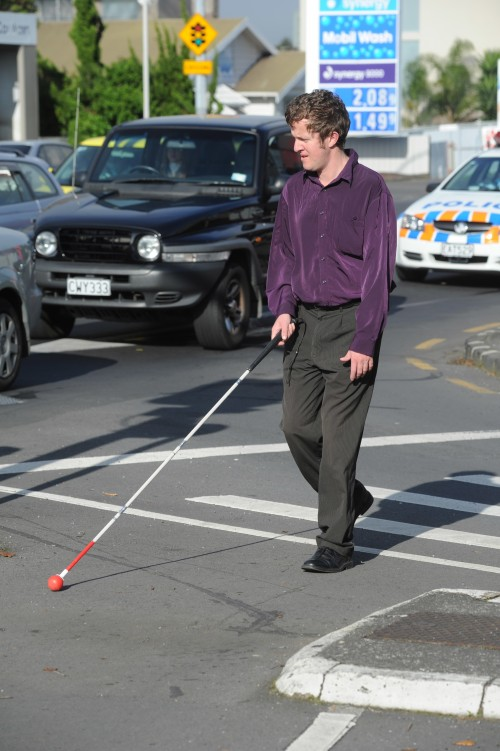
\includegraphics[width=0.3\textwidth]{Images/whitecane.png}
\caption{\label{fig:cane} Blind person on the pedestrian crossing carrying a white cane.}
\label{fig:dog}
\small (Source :\url{http://www.rnzfb.org.nz})
\end{figure}

\subsection{Guide Dogs}
\label{sec:guidedog}

The guide dog is a useful primary 
navigation tool for blind people. 
The guide dogs are trained to 
guide their users around hazards, negotiate traffic, 
locate common destinations 
such as the supermarket, post shop, travel on buses etc
(~\citet{dog1}).  
However, guide dogs are not capable of 
guiding the people in unknown environments 
especially in buildings. 
The blind user therefore does the directing, 
based upon skills acquired through 
previous mobility training. 


The first guide dog training school was established in 
Germany during World War I, to enhance the mobility of 
returning blinded veterans.
Later years have seen the establishments of such 
schools all over the world such as Australia, New Zealand, England etc.
There are about 240 working guide dogs in 
New Zealand (~\citet{dog2}).

The main problem with the guide dog is the 
associated cost which goes beyond 
US\$ 42,000 (~\citet{dog3}). 
This cost includes training the dog and 
providing instructions to the guide dog user. 
Blind people organizations use donations 
to prepare guide dogs and provide to blind people 
for free which limits the availability of guide dogs. 
Due to this reason, white canes are alternatives 
for reasons of price and in case of some people 
with allergies. Today, most blind people still use canes 
at least sometimes, some prefer guide dogs only 
and some use both as shown in Figure \ref{fig:dog}.   





\begin{figure}[h!]
\centering{} 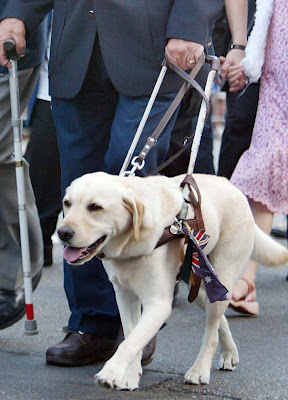
\includegraphics[width=0.2\textwidth]{Images/guidedog.jpg}
\caption{\label{fig:guidedog} Blind person along with a guide dog 
and holding a white cane.}
\label{fig:dog}
\small (Source :\url{http://theexistenceofournaturalenvironment.blogspot.co.nz/})
\end{figure}


\subsection{Miniguide}
\label{sec:miniguide}

Miniguide is a secondary travel aid 
to detect obstacles on the way. 
It is light weight, hand held and 
pocket size device as shown in Figure \ref{fig:miniguide}.
The device uses ultrasonic echo-location 
to detect the obstacles or objects whilst blind person 
navigates. The aid vibrates to indicate the distance to objects 
i.e. a faster vibration means that the object is nearby. 
The device can be adjusted to detect obstacles within different 
distance ranges e.g. 1 meter, 2 meter etc. However, 
only large objects can be detected at 
4 meters or beyond, for example, fences, walls.


\begin{figure}[h!]
\centering{} 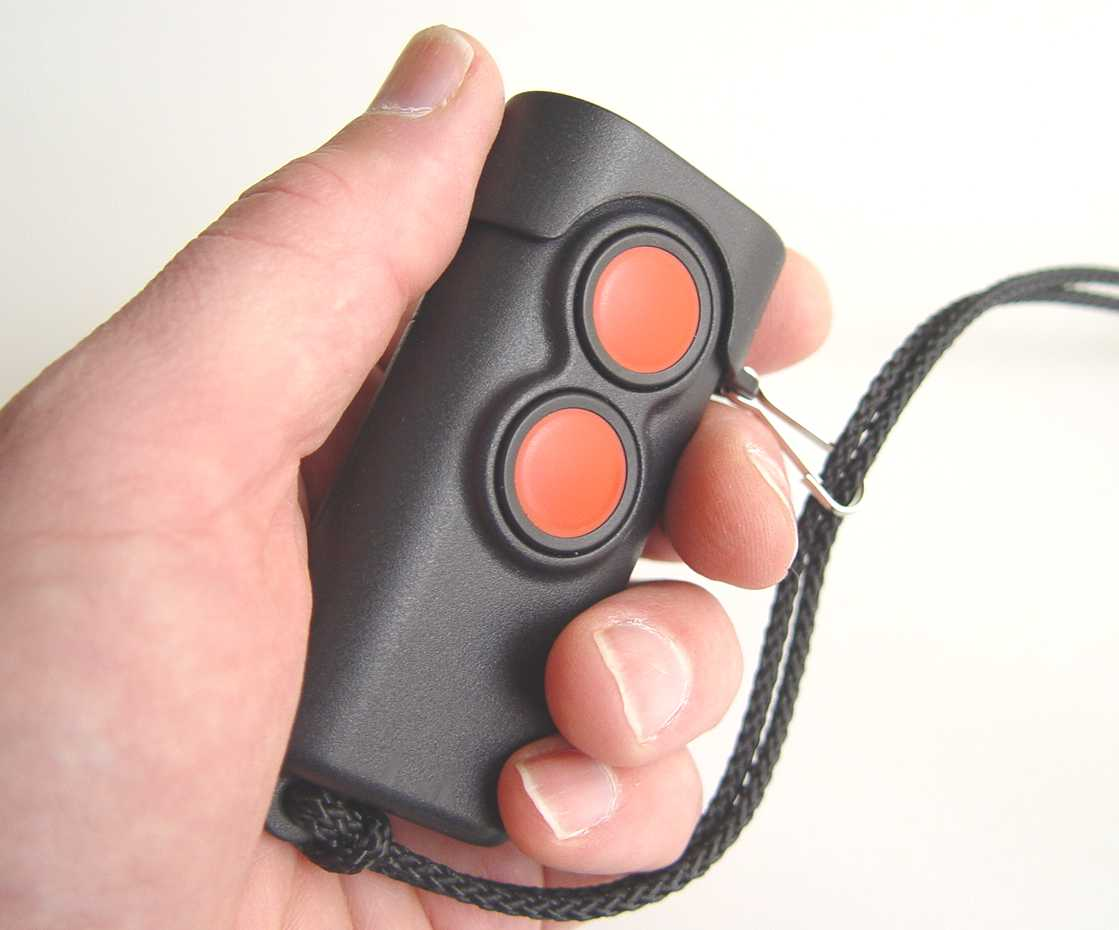
\includegraphics[width=0.2\textwidth]{Images/miniguide.jpg}
\caption{\label{fig:miniguide} Person holding a miniguide.}
\small (Source :\url{http://www.gdp-research.com.au})
\end{figure}

Miniguide has assisted blind people in 
many ways such as avoiding obstacles, 
detecting overhanging obstacles 
(tree branches), locating door ways etc. 
With all these merits, it cannot detect drop offs and 
the cost of miniguide is up to US\$ 400 which 
make sit hard for blind people to afford it (~\citet{miniguide}).

\subsection{Soundpost}
\label{sec:soundpost}

Soundpost is a primary navigation tool. It is 
basically an orientation device and uses 
infrared technology to guide the blind person 
to move accurately from one landmark to the 
other (~\citet{povidi}). It allows 
a blind person to cross up to 
30 meters of an open space. Soundpost uses multiple base stations for generating 
signals and blind person carries a hand held transmitter to 
receive the signals as shown in Figure \ref{fig:soundpost}.
The transmitter starts vibrating once it comes within range 
of a base station and keeps on vibrating until 
you move towards the landmark. 
The transmitter can also generate 
a voice message indicating the landmark information. 


\begin{figure}[h!]
\centering{} 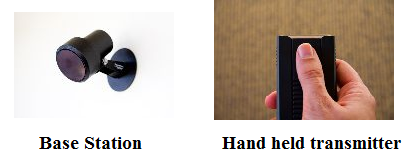
\includegraphics[width=0.5\textwidth]{Images/soundpost.png}
\caption{\label{fig:soundpost} Soundpost device.}
\small (Source :\url{http://www.povidi.com/SoundPost.html)}
\end{figure}

  
A small independent trial is undertaken at the 
University of Canterbury, New Zealand to assess its 
utility for a blind citizen. It has been preferred by both 
guide dogs and white cane users as it further assists 
the navigation in any environment. However it suffers 
from following problems which limit its applicability:-

\begin{itemize}
\item The infrared signal is often broken 
which pose problem during the navigation.

\item It's hard to estimate the 
movement direction towards the landmark 
once the vibration starts.

\item The voice messages are limited.

\item It costs about US\$500 which includes 
the transmitter and two base stations.
\end{itemize}


\subsection{Loadstone GPS}
\label{sec:loadstone}

Loadstone GPS is a free open source software 
for satellite navigation for blind users (~\citet{loadstone}). 
The software currently runs on different 
Nokia devices and requires a GPS receiver.
This project was initiated by Monty Lilburn and 
Shawn Kirkpatrick back in 2004 who are 
themselves blind. The whole program is under the 
General Public License (GPL) and is financed 
entirely by the private developers and by the donations. 
It was made public in 2006 and has been 
a success since then.

The maps consist of way points imported from 
the common map data bases. In some 
cities, rural regions etc no 
exact map data is available in 
common map databases. In such scenarios, 
the software provides users an option to 
create and store their own way points 
for navigation and share it with others. 
There is also a website which allows users 
to share there custom points with each other
and points can then be easily added to the map. 



This application is useful to search for specific locations 
in a given area. However, it lacks some of the 
basic features such as automatic download of maps 
and a route planner. Still tool is very accessible and 
useful when travelling in an area.
\subsection{Research Projects}
\label{sec:research}

In the above sections, we discussed some 
commercial products which provide mobility aid 
to the blind people. A lot of research 
has been carried out in the last few years 
to propose the reliable navigation tools. 
Some of the well known research projects 
which use computer vision and other 
technologies to aid the blind 
user mobility are discussed in the 
following sections. 

\subsubsection{Drishti}

Drishti is a navigation system capable 
of guiding and helping the blind people 
to travel safely both in indoor and outdoor environments (~\cite{ran04}). 
It uses a precise position measurement system, a wireless 
connection, a wearable computer, and a vocal communication interface. 
For outdoor, it uses differential GPS as its location system
to keep the users as close as possible to the 
central line of sidewalks of campus and downtown areas. 
The user can switch the system mode from an 
outdoor to an indoor environment with a simple vocal command. 
An ultrasound positioning system is used to 
provide precise indoor location measurements 
with an accuracy of 22 cm. The user gets 
alerts in the form of vocal prompts to avoid 
the possible obstacles. 
It performs dynamic routing and rerouting to provide 
its blind users with an optimal route for navigation. 
A step-by-step walking guidance is provided for 
navigation in environments. The proposed system is 
good but it is not easy to use as blind person 
have to carry a number of devices.



\subsubsection{Crosswatch}
(~\cite{james08}) presented Crosswatch,
a real time mobile application 
to detect the zebra crossings in outdoor environments. 
At the proposed time, this was the first 
portable system capable of providing 
the real time orientation information 
at urban traffic intersections. 
The system first extracts the straight line segments 
as features from the mobile image. A factor graph model 
is then used to group the features into figure and ground, 
representing crosswalk and background respectively. 
The detection of enough features having sufficient length 
indicates the detection of a cross walk 
and a brief audio tone is sounded for frames 
in which a crosswalk is detected. 
Nokia N95 mobile phone is used in experiments 
which can process approximately three frames per second.
The application is tested with blind subjects to test the usability 
and the subjects answered correctly whether a zebra crosswalk 
is present or absent at all used intersections. 



 (~\cite{james10}) further extended Crosswatch 
to incorporate the detection of 
walk lights on the pedestrian crossings.
Crosswatch is now capable to alert the user 
once the green walk light is illuminated at the intersections. 
Corsswatch is robust, easy to use and performs well in urban 
intersections in the United States.


\subsubsection{Electro Neural Vision System (ENVS)}
(\citet{meers05}) presented ENVS, a system capable 
to avoid obstacles, perceive landmarks 
and assist in navigation via visual sensors, 
GPS and electro-tactile stimulation. 
ENVS first extracts the depth information from the
environment via disparity map 
obtained from the head mounted stereo cameras as shown in 
Figure \ref{fig:envs}. 
This range data is then delivered 
to the fingers via electro-neural stimulation to indicate 
the range of objects being viewed by the cameras to the 
user. To perceive the location of obstacles and the 3D structure 
of the environment, user imagines that the hands are held 
in the direction viewed by the cameras, with fingers 
extended and the amount of stimulation 
felt by each finger indicates 
the range of objects in the pointed direction. 

\begin{figure}[h!]
\centering{} 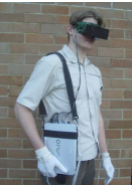
\includegraphics[width=0.3\textwidth]{Images/envs.png}
\caption{\label{fig:envs} The Electro- Neural Vision System.}
\small{Source: (~\citet{meers05})}
\end{figure}

In order to perceive landmarks, 
ENVS uses a GPS, a digital compass and a database of landmarks. 
The relative location of significant 
landmarks is determined (using GPS and stored GPS 
coordinates) and delivered to the fingers via encoded pulses 
when the landmarks are in the field of view. 
The system does quite well in conveying the 
3D structure of the environment to the blind people. 
The experimental results indicate that ENVS 
enables the user to achieve localization, 
obstacle avoidance and navigation without using the eyes. 
However, it is not easy to use because 
blind user needs to carry a laptop and wear gloves 
for ENVS.


\section{Summary}
The purpose of this chapter was to provide a 
overview of navigation system requirements 
and highlight the importance of indoor localisation 
for blind people. Some popular navigation tools along 
with the research projects which aid 
the navigation process are discussed. 
In the next chapter, we discuss the navigation
systems which mainly use computer vision 
techniques such as features, topological maps, 
scene localisation to provide navigation in indoor environments.  
Research works addressing the scene localisation 
problem in indoor and outdoor environments
are presented towards the end in the next chapter.





%
%\begin{enumerate}
%\item \textbf{Pedestrian crossing guidance} 
%\item \textbf{Curbs/Holes identification on the track}
%\item \textbf{Sign boards classification}
%\item \textbf{Temporary hazards identification}
%\item \textbf{Key destinations identification}
%\item \textbf{Voice accent understanding}
%\item \textbf{Location recognition}
%\item \textbf{Obstacle avoidance}
%\item \textbf{Toilets gender categorization}
%\item \textbf{Scene description}
%\item \textbf{Stairs guidance}
%\item \textbf{Guidance in corridors}
%\end{enumerate} 

%
%\section{Indoor Navigation Systems}
%Simultaneous localization and mapping (SLAM) is a 
%technique used by robots and autonomous vehicles 
%to build up a map within an unknown environment (without a priori knowledge), or to update a map within a known environment (with a priori knowledge from a given map), while at the same time keeping track of their current location.
%
%Indoor navigation systems are based on different technologies 
%such as WIFI, laser range etc. Each technology used for 
%indoor navigation system has its pros and cons. Some commonly used 
%technologies for indoor navigation system are as follows:-
%
%\subsection{Using Laser Scanner} 
%In indoor, the localization using laser range 
%finder has been used a lot. However these 
%methods provide a 2D map of the environment. 
%
%The navigation system these days are based on different technologies.
%Every technology has it pros and cons.
%
%\subsection{With WIFI Fingerprints}
%\subsection{With Images}
%\subsection{With Smartphones}


%\section{Visual Navigation}
%\label{sec:visualnavigation}
%
%The vision (image or videos) has become common in applications 
%such as localisation, automatic map construction, 
%autonomous navigation, path following etc in the 
%last few years. The navigation techniques based 
%on vision increase the scope of application of autonomous 
%mobility and have resulted in countless research 
%contributions for robots, autonomous ground vehicles, 
%unmanned aerial vehicles and blind people. 
%The systems that use vision for navigation can be 
%divided into two main categories:-
%
%\subsection{Map based systems}
%\label{sec:mapbasedsystem}
%
%This include those systems that either 
%need to have some representation of the environment 
%before the start of navigation process. 
%There are three systems 
%mainly (1) systems that need a complete map 
%of the environment before hand referred as \emph{map-using}, (2) systems that explore the environment 
%and automatically build a map off line referred as \emph{map-building}, and (3) systems that perform 
%the map construction online referred as \emph{local map-based}.
%
%In \emph{map-building} approaches, precise localization is important 
%for accurate map building and is the must needed functionality. 
%In standard \emph{map-building} systems, it is assumed that localisation 
%can be computed by some other techniques. However in 
%pure localisation approaches the map is presumably 
%available and systems need to track its own position and orientation in 
%the environment continuously. If the exploration and mapping of an 
%unknown environment is done automatically online, the navigation system 
%needs to explore, map and localise itself simultaneously usually 
%referred as Simultaneous localization and mapping (SLAM). 
%Recently, cameras have been used as the sole sensor
%yielding visual SLAM (~\citet{chen07, davison07}). In this section, 
%we discuss vision based navigation systems with a 
%that belong to one of the three mentioned categories 
%and work in indoor environment.
%
%Sim \emph{et al.} presented a system that is capable of
%mapping a large, complex visual environment in real time using 
%a pair of stereo cameras (~\citet{sim06}). 
%The system explores, navigates autonomously and
%generates a hybrid map representation that facilitates the 
%accurate localization (using visual landmarks) and safe
%navigation (using occupancy grids). The landmarks are 
%detected in images using the SIFT features (~\citet{lowe04}), 
%matched using best bin search and are stored. 
%This is followed by an occupancy representation 
%to obtain a reliable spatial representation 
%of the world to ensure real time safe navigation. 
%They used an Activmedia Powerbot robot 
%with a stereo head. The robot explored and 
%did well in a laboratory environment
%consisting of two rooms of total size approximately
%19m by 16.5m.
%
%A topological map is a graph based representation 
%of the environment where each node corresponds to a 
%zone of the environment and can be associated with 
%action such as turning, crossing a door etc.
%Gaspar \emph{et al.} used omnidirectional camera 
%to create a topological map of the indoor structured 
%environment during a training phase (`\citet{gaspar00}).
%The insect vision based capability was emulated allowing the system to advance 
%along corridors, recognize the ends, turn into correct directions 
%etc. Each node is recognizable with landmarks and covers the movement 
%between the two nodes for instance two doors joined by a corridor.
%
%Kidono \emph{at al.} developed a system which needs human guided 
%pre-training phase (~\citet{kidono02}). 
%A human guides the robot through an environment 
%and during this guided route, the robot records images 
%with a stereo camera. The recorded images are used 
%to construct a 3D map on line incrementally 
%frame by frame. Once the map is built, the robot can 
%repeat the same route from the starting point to the 
%goal point, tracking features and computing 
%the closes safe path. The robot was
%navigated in an indoor environment and performed well.
%
%
%
%Anther important application of map building navigation systems 
%are the museum guiding robots. These robots need to be autonomous 
%to recognize people, guide them through different environments 
%and also avoid obstacles. Thrun \emph{et al.} developed a robot 
%MINERVA that uses two cameras combined with a laser sensor 
%to build map of the environment for the navigation process (~\citet{thrun99}).
%MINERVA uses laser scans, camera images and odometry 
%readings to build the occupancy and texture maps 
%via joy-sticking the robot through its 
%environment during training phase. Texture maps
%of the ceilings are generated using image mosaics 
%to handle the crowd with in the museum.
%The robot remained operational for two weeks 
%Smithsonian’s National Museum of American History 
%and successfully interacted with thousands of people.
%Shen \emph{et al.} proposed ATLAS, a museum 
%guiding robot that combines topological map building 
%image matching algorithms for localisation (~\citet{shen06}). 
%The robot is designed to detect the nearby visitors nearby 
%and interact with them via voice and a touching screen. 
%Moreover, system also incorporates a human face detection 
%algorithm to actively approach to new visitors.
%
%The approaches discussed so far are based on global 
%description of the environment which can be either obtained
%automatically or by a human guided stage but before the start 
%of navigation. Since the early nineties, some 
%authors have developed the navigation systems 
%which support on line construction of a local 
%occupancy grid. The local grid refers to the portion of 
%the environment surrounding the robot and grid size is
%determined by the camera field of view. This local information 
%is used for a subsequent map construction frame by frame 
%for on line safe navigation. Gartshore \emph{et al.}
%presented a system capable of building maps from online images 
%captured by a single camera.  The systems computes the 
%probabilities of finding the objects at every location. 
%The algorithm detects the object boundaries using edge and 
%corner detector. Detected features are back 
%projected from the 2D image plane considering all the potential locations 
%at any depth. The system computes the position using odometry 
%data combined with feature extraction process. Color or gradient 
%from edges and features from past images 
%help to increase the confidence of the object presence 
%in a certain location. The experiments were conducted 
%in indoor environments and robot moved 100mm between consecutive images.
%
%In the recent years, visual sonar is also used 
%for the navigation purposes. It uses range data and depth measurements 
%for navigation purposes in an analogous way to 
%ultrasound sensors. Martin used the same idea 
%to compute depth from single camera images of indoor 
%environments (~\citet{martin06}).
% The genetic programming is used to 
%discover the best algorithm to detect the ground boundaries 
%in a training phase. These algorithms then use obstacle 
%avoidance strategies initially developed for sonar.
%The algorithms are designed to be a 
%replacement for sonar, returning the location of
%the nearest obstacle in a given direction. The three 
%indoor data sets were used with a total of 
%images from four different hall ways.
%
%\subsection{Mapless systems}
%These refer to those techniques which do not need 
%any knowledge of the environment but they navigate 
%as they perceive the environment. These techniques 
%often grab video frames to produce enough information 
%about the unknown environment and navigate through it 
%safely. 
%
%Optical flow is one of the technique commonly used 
%for mapless systems. It can be defined as apparent motion 
%of features in a sequence of images i.e. video frames.
%Taludker \emph{et al.} (~\citet{talukder04}) 
%presented optical flow based 
%solution to detect the dynamic objects in the camera field of view.
%The system assumes that dynamic objects create discontinuity 
%in optical flow orientation and changes in magnitude with respect to the 
%background pixels optical flow direction and magnitude. The system 
%is tested using a single camera and later enhance with a stereo camera.
%
%Green \emph{et al.}  (~\citet{green03}) 
%described the design of a robot that can fly in 
%the buildings controlled by an insect inspired optical flow based system. 
%The relevance of insect based navigation strategy in an optical flow 
%based navigation was emphasized in the work.
%
%
%Appearance based navigation strategy record images or 
%prominent features of the environment as model templates. The 
%models are basically labeled with a certain location information. During
%navigation stage, the robot matches on line image with stored images. 
%The main problems with such approaches are (1) how to create environment 
%representation (2) performing the online matching criteria. 
%In such techniques, loop closure i.e. detection of previously 
%recorded images plays an important part during the navigation 
%phase. 
%
%Zhou \emph{et al.} (~\citet{zhou03}) 
%utilized histograms based on color, gradient, 
%edge density and texture to describe the appearance 
%of trained images. The recognition during online stage is 
%performed by matching the histogram of query image with the 
%stored templates. 
%
%Remazeilles \emph{et al.} (~\citet{remazeilles04}) used an appearance based navigation 
%system. The system uses an image data base which is a set of views 
%built off line representing the whole navigable environment.
%Once navigation mission is defined, an image sequence corresponding to 
%what robot should see during the motion is extracted from the data base.
%The robot motion is the result of online detection and matching 
%process between the models included in the sequence and 
%perceived scenes.To navigate, the robot tracks recognizable previously cataloged 
%features.
%
%Fraundorfer \emph{et al.} (~\citet{ fraundorfer})proposed vision based localisation and mapping 
%for robot navigation. The environment is represented as a linked 
%collection of way point images. The collection is built online while 
%robot is exploring the environment.  Links are created between the 
%sequential images and are inserted by image matching. 
%An efficient image matching scheme allows real time mapping and global 
%localsation. 
%
%Booji \emph{et al.} (~\citet{booji}) 
%proposed navigation via image based topological map. 
%The robot is driven through the environment and keeps on 
%taking the pictures. The system uses epipolar constraints 
%based on SIFT features to match the images. By conputing the 
%similarities between these images a topological map 
%in form of in form of an appearance graph is created.Navigation on 
%this graph involves heading from one node to the other.
%
%Se \emph{et al.} (~\citet{se01}) proposed a vision based localisation and mapping 
%algorithm which uses scale invariant image features as landmarks in unmodified 
%dynamic environments. The 3D landmarks are localised and robot 
%ego-motion is estimated by matching them 
%taking into account the feature viewpoint extraction.
%
%Feature tracking navigation systems tracks features 
%in consective frames to perform the navigation. 
%Pears and Liang \emph{Et al.} (~\citet{liang02}) 
%use hoographies to track ground plane corners 
%in indoor buildings.  The same authors extended their 
%work by using homographies to calculate the height of 
%tracked features or obstacles above the ground plane during the navigation. 
%
%During robot driving throught the environment, SIFT based methods extract 
%the important features from the environment which 
%serve as landmarks to be tracked for navigation, global 
%localisation and robust vision based SLAM performance 
%(~\citet{se02, se05}).
%%\begin{itemize}
%%\item \textbf{Map based navigation:} 
%%These systems require a map of the environment 
%%for the navigation. It also includes those systems that can explore the environment 
%%and build the map by themselves. However 
%%the environment needs to be explored first 
%%and its representation is stored before the start of navigation.
%%Therefore systems in this category will start 
%%navigation if and only the environment map 
%%is available.
%%
%%\item \textbf{Mapless navigation:}
%%It includes all navigation approaches that do not 
%%require any knowledge of the environment for navigation
%%run. Navigation is performed on the basis of elements 
%%observed in the environment such as walls, features,
%%doors, desks, etc. 
%%
%%\end{itemize}
%%
%%In the last few years, lot of progress is observed in context 
%%of visual navigation. The older techniques have been refined 
%%and lot of new techniques are also presented 
%%which have led to a more accurate and 
%%efficient navigation systems. We review some of the 
%%visual navigation approaches used for map based and 
%%mapless navigation in the following sections. 
%%
%%
%%\subsection{Map based systems}
%%This category includes systems that need a complete map 
%%of the environment before the start of navigation.
%%Other systems in this category are able to 
%%explore the environment and 
%%automatically build a map. However the navigation 
%%phase will start only once the map is built. 
%%The map information can be directly 
%%used for navigation or it can be
%%post-processed to improve the map accuracy
%%to achieve a more precise localization. 
%%
%% 
%%\section{Visual Indoor Navigation}
%%\begin{enumerate}
%%\item Map based navigation
%%\begin{enumerate}
%%\item Topological maps
%%\item Local maps
%%\end{enumerate}
%%
%%\item Map less navigation
%%\begin{enumerate}
%%\item Optical Flow
%%\item Appearance based navigation
%%\item Feature based navigation
%%\end{enumerate}
%%\end{enumerate}
%
%
%%\section{Simultaneous Localisation and Mapping (SLAM)}
%%A brief discussion about SLAM.
%%\subsection{Visual SLAM}
%%Discussion about SLAM based on images.
%%I will mention some of the research works 
%%based on Visual SLAM for robotics.
%
%\subsubsection{Loop Closure}
%Discuss the importance 
%of loop closure i.e. identification of the place 
%which has been already visited.
%
%
%
%\section{Image based localization}
%I will state that our indoor location recognition is 
%also based on image based localisation.
%We are doing a 2D image base matching.
%I will discuss some research works briefly 
%which have done localisation in indoor environments
%using different techniques based on 2D images.



%
\chapter{Image based localisation}
\label{chap:visualnavigate}
%
%
\vspace{-10.0em}
\begin{abstract}
The previous chapter mentioned some navigation tools 
which assist the navigation. This chapter moves to a 
next level and reviews works which 
offer visual navigation for robotics or 
visually impaired people. The localisation based 
on different technologies is reviewed to understand the 
importance of vision based localisation. 
Finally, we present some good research works 
which use robust computer vision techniques to 
perform scene matching in indoor and outdoor 
environments. 
\end{abstract}



\section{Visual Navigation}
The navigation based on vision (images or videos) 
is referred as "walk through problem". 
The vision sensor seems to be the best choice 
for navigation if we consider its nice features 
like low price, low power, non contact and 
high potential information contents. 
However, its really hard to extract useful 
and reliable information from the image feeds 
to base mobility decisions.
The visual navigation focuses on guidance with the 
goal of automatically reproducing the tasks performed
by humans without any visual impairment. The important tasks 
are to detect the current location, plan the route 
and then guide the blind person safely 
while avoiding the possible obstacles on the way. 
 Francisco \emph{et al.} provides a very good survey 
on visual navigation for mobile robots 
and mention key research contributions 
which are made from nineties till 2008 (~\citet{bonin-font08}).
The visual navigation systems are
divided into two main categories:
% (1)
%map-based systems which need some 
%representation of the environment in 
%the form of a map before the start 
%of navigation, and (2) mapless systems 
%which do not need any map aof the environment. 
%In mapless systems, navigation is 
%determined by observing and extracting
%useful features in the environment 
%based on on board sensors.



\subsection{Map based systems}
\label{sec:mapbasedsystem}

Map based systems need 
some representation of the environment 
built before the start of navigation process. 
There are two systems mainly 
(1) systems which use an existing 
map of the environment 
usually referred as \emph{map-using}, 
and (2) systems that 
build the map of the environment themselves 
usually 
referred as \emph{mup-building}. 
The navigation starts only 
after the environment representation or a 
map is available.

%Map building and self-localization in the navigation environment 
%are two functionalities that most systems tend to incorporate. 
%In standard map-building approaches, 
%the localization in the environment can be computed
%by some other techniques while in pure 
%localization approaches, the map of the
%environment is presumably available. 
For a true autonomous visual navigation, the 
system needs to do automatic exploration, 
localisation and mapping of the environment 
via techniques known as Simultaneous localization and mapping (SLAM).
SLAM basically involves the simultaneous 
estimation of a map and the robot pose concurrently.
%Normally 
%systems based on SLAM solve each of the two 
%problems independently i.e. a robot can trivially 
%estimate its position given a complete map of its environment 
%and it can also construct a map from sensor data if i
%ts position is accurately known. 
Recently, cameras have been used as the sole sensor
to yield SLAM based on vision i.e. visual SLAM (~\citet{chen07, davison07,silveira08}).
A standard scheme to visual SLAM consists 
of first extracting a sufficiently
large set of features and robustly matching
them between successive frames. These corresponding features
are used for estimating the camera pose
and scene structure. In this section, 
we discuss some well known SLAM systems 
which make use of a map 
with a particular focus on indoor buildings. 
%with a focus on indoor buildings.

Davison presented MonoSLAM which 
is based on monocular vision and is one of the most 
successful schemes for a single camera (~\citet{davison03}). 
Landmark positions and camera pose 
are estimated and refined directly from 
observations in the image using an 
Extended Kalman Filter (EKF).
The camera can be positioned accurately 
for extended periods provided that sufficient landmarks 
are tracked. However, the positioning is limited to 
small scale environments with 100 
landmarks in total. Clement \emph{et al.} 
(~\citet{clemente07}) 
extended MonoSLAM to deal with 
larger environments by using 
the submaps framework proposed by (~\citet{estrada05}).
MonoSlam is used on small scale and new map is started 
once the number of landmarks grows beyond
some limit. The local submaps are combined into 
an accurate global map by opimising transformations 
between submaps. The system is able to close 
250m loop with an accurate global map.



Sim \emph{et al.} presented a system which maps 
a large and complex environment in real time using 
a pair of stereo cameras (~\citet{sim06}). 
The main contribution of the work 
is a fully automatic mapping system which operates 
on-line and consistently produces accurate maps of 
large scale environments. The system uses a hybrid approach 
consisting of 3D landmark extraction based on 
SIFT features (~\citet{lowe04}) for 
image localisation and occupancy grid 
to obtain a map for a safe navigation. 
The occupancy grid represents
the environment as an evenly spaced 
field of binary random variables each 
representing the presence of an obstacle 
at that location in the environment.
The occupancy grid offers a reliable 
spatial representation of the 
world for a safe navigation. 
The proposed system is deployed on 
a robot and it does well in a laboratory 
environment with of two rooms during the testing. 


%A topological map is a graph based representation 
%of the environment and is often used for navigation. 
%Each node corresponds to a place in the environment 
%and is associated with actions 
%such as turning, crossing a door etc.
Topological maps are graph based representation 
of the environment and are 
parsimonious representation because they are 
simple and easy to scale. Winters \emph{et al.} (~\citet{winters99} 
proposed a system for robot which 
uses omnidirectional camera images to generate a 
topological map of the indoor structured 
environment during a training phase.
The links in the graph are sequence of images 
belonging to a place (e.g. corridor) and nodes 
represent specific places associated with actions 
such as turning, crossing a door etc. 
The image set is represented by %compressed by %compressed by Principal Component Analysis to obtain 
a low dimensional eigenspace and robot determines
its position by projecting the current image into eigenspace 
during movement. After position estimation, 
the robot uses ground plane images to extract 
corridor guidelines to control its trajectory. 
The system does well in corridors of 
Institute for Systems and Robotics, Portugal (ISR) 
\footnote{\url{http://welcome.isr.ist.utl.pt/home/}}.


Kidono \emph{at al.} developed a system 
which needs training from a human to build a map (~\citet{kidono02}). 
As user guides a mobile robot to a
destination by remote control, 
the robot constructs a 3D model on line incrementally 
frame by frame from stereo images. 
For autonomous movement, the robot 
utilizes the map and past experience on observation 
to safely navigate from the starting point 
to the goal point.  The robot is navigated through an 
indoor room with different obstacles and did well.
%. During this movement, the robot observes the surrounding
%environment to make a map. Once the map is generated, the robot computes and follows
%the shortest path to the destination autonomously. To
%With the map, 
%the robot can can repeat the sane route from 
%starting point to the goal point via tracking the features 
%and finding the closest safe path. 



%Anther important map building robot applications are 
%the museum guiding robots which need to be autonomous 
%to recognize people, guide them through different environments 
%and also avoid obstacles. 
Thrun \emph{et al.} developed a museum guiding robot 
MINERVA\footnote{\url{http://www.cs.cmu.edu/~minerva/}} that uses laser scans, camera images and 
odometry readings to to build map of the environment for 
the navigation (~\citet{thrun99}). The robot is first navigated 
via joystick in the museum to generate 
occupancy and ceiling texture maps. The occupancy 
grid ensure safe navigation and texture maps are used 
for localisation in case of a huge crowd because 
frontal images do not offer sufficient information for 
feature based tracking. The robot remained operational for two weeks 
at Smithsonian’s National Museum of American History 
and successfully interacted with thousands of people.
Shen \emph{et al.} proposed ATLAS, a more advanced 
museum guiding robot (~\citet{shen06}). 
The laser data and images are used 
to match the map data of the environment for localisation. 
A visual appearance based algorithm is than used for normal
topological navigation. In visual appearance algorithms, 
the current image is compared with stored templates or models 
for the recognition. ATLAS is tested in the foyer of London County
Hall for 03 months. The robot can (1) detect the nearby visitors 
and interact with them via voice and a touching screen, (2)
uses a human face detection to approach to new visitors
and (3) can detect the battery level and
charge itself automatically. This makes ATLAS possible to
run continuously in a museum environment.


%The approaches discussed so far use global 
%description of the environment obtained either 
%automatically or by a human guided stage before the start of navigation. 
Some navigation systems support on line construction of a local 
occupancy grid which is the portion of 
the environment surrounding the robot.
This local information is used for a 
subsequent map construction frame by frame 
for on line safe navigation. 
Gartshore \emph{et al.}
presented a framework for map building 
based on online images captured by a single camera
 (~\citet{gartshore02}). 
%The work focuses on locating the 
%position of features in 
%the environment during the map building.
The main contribution of the work 
is combination of occupancy 
grid and visual data from a single camera.
The system uses feature detector 
algorithm to identify the object boundaries 
based on features in occupancy grids 
from the current frame. While positioning 
module computes robot position using 
odometry data and detected features. 
The color or gradient from 
features from past frames are used 
to further verify the object presence 
at a specific location. 
%The systems computes the 
%probabilities of finding the objects 
%at every location. The edge features are used to detect 
%object boundaries for the current frame.
%The positioning module of the system computes the 
%position of robot via odometry data and 
%with extracted features. The color or gradient 
%from edges from past frames help to verify the 
%object presence at a certain location. 
The experiments were conducted in indoor environment 
and robot was able to navigate safely while 
avoiding the obstacles. 

Botterril \emph{et al.} presented a BoWSLAM scheme 
which enables real-time navigation of robots 
in dynamic environments using a single camera alone 
(~\citet{botteril10}).
The robot can position itself in real-time while exploring 
a previously unknown environment. 
The system works by representing 
every frame as a Bag of Words (BoW). BoW 
representation is then used to select 
multiple nearby frames to compute relative positions 
and latest frame is positioned relative to each of these 
frames. A subset of these multiple position hypotheses 
with minimum gross errors is selected 
to accurately position the robot in a global
map. The proposed system allows robot navigation in 
challenging dynamic and self-similar environments.


\subsection{Mapless systems}
These systems refer to those techniques which do not need 
any knowledge of the environment but they navigate 
as they perceive the environment. These techniques 
often grab video frames to produce enough information 
about the unknown environment for a safe navigation. 

Optical flow is one of the technique commonly used 
for mapless systems. Taludker \emph{et al.} presented 
a novel optical flow based solution 
for robots to detect the presence of dynamic objects 
in the camera field of view during navigation (~\citet{talukder04}).
The algorithm assumes that moving objects cause discontinuity 
in optical flow orientation and changes its magnitude with respect 
to the background pixels orientation and magnitude.
The system is initially tested with single camera and 
later on with stereo cameras to extract the depth information.


Green \emph{et al.} presented a Closed Quarter Aerial Robot (CQAR) 
whose navigation is controlled 
by an insect inspired optical flow based system  (~\citet{green03}) . 
The robot can fly into buildings, take off and land 
based on optical flow computed from the images 
of the environment. The minimum flying speed of 
CQAR is 2 m/s and it needs to turn
%, the turning radius is about 2.5 m and it needs 
5 meters before to avoid an obstacle. 

 Zhou \emph{et al.} used appearance based strategy 
for mapless navigation  (~\citet{zhou03}). Such strategies 
has two phases (1) first in a pre-training phase,
the images or prominent features from the environment 
are observed and stored as model templates. 
These models are labeled with a certain location 
information, % or with an associated control steering command, 
and (2) in the navigation stage, the
robot matches the current image with the stored templates 
to recognize the environment and self-localize. 
Zhou \emph{et al.} 
utilized color, gradient, edge density and texture 
histograms to describe the appearance of pre-recorded 
indoor images. The navigation is performed by matching 
the multidimensional histogram of current image with 
the stored templates. The use of histograms save 
computation resources and are simple to use.
The main problems with appearance based strategies are
to identify the ways to represent the environment 
and perform on-line matching. 

The image qualitative characteristics and their interpretation 
are often used by visual techniques to navigate 
and avoid obstacles. The navigation systems 
based on qualitative information avoid as
much as possible the obstacles in the environment. 
%The are two types of reactive visual obstacle 
%avoidance systems (1) model-based systems, 
%which need pre-defined models of known objects, and 
%(2) sensor-based systems, which process 
%every online sensor information to determine the 
%free space and obstacles. 
Fasola \emph{et al.} proposed to use 
image color segmentation techniques 
to detect the possible objects from frames 
followed by classification of opponent robots 
via gray scale umage processing (~\citet{fasola06}). 
The integral images which were introduced for real time 
face detection have been used for a robust robot classification 
(~\citet{viola01}). The proposed system is developed
with the annual RoboCup Competition in mind 
where teams of Sony AIBO 4-Legged robots compete
in the game of soccer. From a set of 327 test
images, the system was able to achieve a 97\% 
classification accuracy yielding only one false positive.


The techniques for tracking moving elements 
in a video sequence have become robust enough and useful 
for navigation. Such techniques divide a tracking task into two sub-tasks
(1) motion detection, which refers to the identification 
of most likely region in next frame to find the feature, 
and (2) feature matching, by which the 
feature tracked is identified within the determined region (~\citet{trucco06}).
Such techniques do not handle the obstacle avoidance.
SIFT features (~\citet{lowe04}) are the popular features 
for the navigation so far. During the navigation, the 
SIFT features are observed from different viewpoints, angles, distances 
and with different illumination changes. The detected features serve as 
appropriate landmarks to be trace over time for navigation, 
global localisation and a robust vision based SLAM performance 
(~\citet{se01, se05}).

Saeedi used stereo vision in a novel navigation strategy applicable to unstructured
indoor/outdoor environments (~\citet{saeedi06}). 
The main emphasis of this work is to estimate the robot motion
independently from any prior scene or landmark knowledge. 
The system uses a new, faster and more
robust corner detector and detected features are 3D positioned.
The 3D positions of scene features and the robot 
are refined by a Kalman filtering over time. The results 
indicate a good tracking and localization performance covering 
outdoor environment of 5 cm by the system.

\section{Localisation}
\label{sec:localisation}
In the previous section, we have reviewed 
some key contributions in area of visual navigation 
for robotics. However, same techniques can be utilized 
for blind people by replacing the control signals 
with appropriate voice messages.
 
However, the focus of our work is the scene localisation 
in indoor environment only and not the navigation. 
Technologies other than vision have been used 
for indoor positioning, such as infrared,
ultrasonic etc. It is important to briefly review these techniques 
to understand the corresponding limitations to 
identify the benefits of vision based localisation. 
In this section, we briefly discuss indoor positioning based on 
different techniques for the analysis (~\citet{indoorsurvey11, gu09}). 


\subsection{Infrared}
\label{sec:infrared}
Infrared (IR) positioning technology needs infra-red 
emitters and measures the position of the object
according to the receiving time of infrared signals. 
Want \emph{et al.} developed Active Badge system, one
of the first successful IR based indoor positioning system at
AT\&T Cambridge in 1990s  (~\citet{want92, harter02, abs08}). The person needs 
to carry an active badge and system provides room level 
indoor localisation with active badges.
An active badge transmits a globally unique IR signal every 15
seconds. In each located place, one or more sensors are fixed 
and detect the IR signal sent by
an active badge. 
The position of an active badge can be
specified by the information from these sensors 
and forwards the location information
of the tracked active badges to a central server.
The price of active badges and networked sensors
are cheap but the cables connecting the 
sensors raise the cost of the
Active Badge system. 
%Moreover, the effective transmission 
%range of this positioning technology is
%only a few meters since the poor penetration of infrared.
%The system may not work well in glass structure buildings as 
%it is influenced by sunlight and fluorescent.

OPTOTRAK system is designed for positioning in 
congested shops and workspaces ~\cite{opo08}. The OPTOTRAK
uses a system of three cameras as a linear array to track 3-
D positions of numerous markers on an object. 
The markers mounted on different parts of a
tracked object emits IR light which is detected by the camera
of the system to estimate the location of them via triangulation 
technique. The system offers a high accuracy of 0.1 mm to 0.5 mm
with 95\% success probability. A disadvantage of OPTOTAK system
is the line-of-sight requirement between the objects and the
tracking system. However this can be partially solved 
by using a large number of IR markers at the expense of cost. 

IR based systems provide a precise position estimation 
%IR emitters are small, light-weight and the system 
%architectures are simple leading to a low 
%installation and maintenance cost. However, there 
%are still some disadvantages with these systems. 
However, IR signals have some limitations for sensing location, 
for example, interference from florescent light and sunlight. 
This problem can be solved by using optical and electronic filters 
but it raises the cost of the positioning system. 
Although, the IR emitters are cheap but whole system using camera array, 
transmitters, IR device and wire connectivity for each isolated 
place increases the cost of system.
connected via wires is expensive when used in large areas. 
%comparing to the coverage
%area. There should be a transmitter or receiver in every
%measured place such as a room equipped with at least one IR
%device to locate whether the target persons or devices are in
%the room or not. These transmitters or receivers fixed in each
%place are connected using special wire. In addition, when an
IR device taken by a person is covered by his/her clothes,
the system fails to work since the IR wave can not penetrate
opaque materials.

% developed ActiveBadge, 
%one of the best indoor positioning 
%working system so far. The system got refined 
%with time. Each user needs to carry small infrared
%marking equipment. The marking equipment sends a globally unique identification
%code every 15 seconds and infrared sensors 
%fixed in the building collect the data
%then transmit to a central server which accomplishes the positioning process. 
%ActiveBadge is low cost and easy to use, but it is 
%vulnerable to the impact of fluorescent and
%sunlight. Moreover, the effective transmission 
%range of this positioning technology is
%only a few meters since the poor penetration of infrared.
%The system may not work well in glass structure buildings 
%due to sunlight coming through the windows. The associated 
%cost is also higher. The largest single system is at Cambridge University Computer Laboratory, 
%where over 200 badges and 300 sensors are in daily use.

\subsection{Ultrasonic}
\label{sec:ultrasonic}
Using ultrasound signal is another way to measure the position. 
Ultrasound signals are used by bats to navigate
in the night which inspire people to design a similar navigating
system. Ultrasonic positioning technology uses mainly reflective distance method to
determine the location of the object. 

Active Bat system is a well known 
ultrasonic indoor positioning system researched by AT\&T Labs (~\citet{ultrasound04}).
It is a low-power, wireless indoor location system accurate up to 3 cm. 
It relies on multiple ultrasonic receivers embedded in the ceiling 
and measures time-of-flight to them. It works by finding 
the distance to minimum of three reference 
nodes and then using multilateration technique to find the exact position. 
The performance of the system is influenced
by the reflection and obstacles between tags and receivers,
which degrades the system accuracy. The scalability of the system 
is affected due to deployment of 
a large number of sensors on the ceiling. 
The receivers also need to be accurately placed,
which results in complex and costly installation.

Cricket system is another location system which offers 
efficient performance and low cost (~\cite{priyantha00,priyantha05}). 
The cricket system uses time of arrival measuring method
and triangulation location technique to locate a target. The
system includes ultrasound emitters as infrastructure
attached on the walls or ceilings at known positions, and a
receiver mounted on each object to be located.
The cost of the whole system is low and it can 
provide a position estimation accuracy of 10 cm.
The receivers in the cricket system consume more power 
and its power supply needs to be efficiently designed 
to avoid frequent charging.
The Sonitor ultrasound IPS is an indoor tracking
and positioning solution provided by Sonitor Technologies
Inc (~\citet{sonitor08}). The Sonitor system can locate and track people and
devices in real-time and offer very good room level accuracy. 

%Ultrasound positioning systems give a kind of inexpensive positioning
%solutions. Usually the ultrasound signals used to locate
%objects need to be combined with RF signals, which perform
%synchronization and coordination in the system. These ultrasound
%positioning systems increase the system coverage area.
%However, ultrasound-based positioning systems have lower
%measurement accuracy (several centimeters) than IR-based
%systems (several millimeters). These ultrasound positioning
%systems suffer from reflected ultrasound signals and other
%noise sources such as jangling metal objects, crisp packets,
%etc.
 Usually the ultrasound signals used to locate
objects need to be combined with RF signals, which perform
synchronization and coordination in the system. These ultrasound
positioning systems increase the system coverage area.
However, Ultrasonic positioning system requires 
large-scale layout with many of receiver hardware 
leading to a overall higher cost. 
The positioning result is very sensitive with the
environment and suffers from reflected signals, 
metal objects etc. 

%\subsection{ZigBee}
%\label{sec:zigbee}
%
%ZigBee is a short distance, low-rate wireless network technology 
%and achieves positioning with the coordination of 
%communications by thousands of tiny
%sensors. These sensors require very little energy to relay the data passing between the
%sensors leading to a very efficient communication. 
%The accuracy of such systems is limited and systems 
%become unstable with clusters of people. 
%The associated cost is also higher 
%due to use of large sensors.
%Wireless Dragon 
%positioning system is a representative 
%ZigBee positioning system developed by Chengdu 
%Wireless Dragon Communication Technology Co., Ltd. 

\section{RFID}
\label{sec:rfid}

Radio frequency (RF) technologies use frequency signals 
which can travel through walls and human bodies easier
therefore offering a larger coverage area and
less requirement of hardware. The RFID positioning
systems are commonly used in complex indoor environments
and offer cheap identification.


LANDMARCE positioning system is a RFID-based indoor
positioning system developed by Michigan State University and the Hong Kong
University of Science and Technology (~\citet{ni04}). 
The system uses fixed position reference tags and 
%which are placed in a fixed position 
and RFID readers to determine the nearest reference 
%the compare the signal strength from the target and 
%reference tags to determine 
tag from the target tag followed by locaiton estimation. 
%Location can be determined by the nearest reference and reference tags. 
Jin \emph{at al.} further improved LANDMARC with respect to system's energy consumption
and costs (~\citet{jin06}). 

WhereNet positioning system offers indoor and outdoor real-time positioning 
(~\citet{wherenet08}).
RFID technology is used to identify various located tags mounted 
on the target located objects, such as a device or a person.
The system uses differential time of arrival algorithm to 
calculate the precise locations of these tags.
The tags are powered by batteries which can last up to 7
years depending on the transmission rate of the tags. However,
the WhereNet offers an error range around 2 m to 3 m,
which is not very accurate in indoor situations. The system
is complex and the installation of these devices is
time consuming.

The advantage associated with RFID positioning system is light and small
tags that can be taken by people to be tracked. The RFID
system can uniquely identify equipment and persons tracked
in the system. However, the absolute positioning
techniques need numerous infrastructure components installed
and maintained in the working area of an RFID positioning
system which increases the overall cost.

%The disadvantage of such positioning systems is the RF signal
%influenced by the antenna, the role of proximity does not have the communications
%capabilities, positioning coverage is small, and not easily integrated into other
%systems. 

\subsection{WLAN}
\label{sec:wlan}

WLAN technology is very popular and 
is widely used in business districts, universities, airports etc. 
WLAN-based positioning systems reuse the
existing WLAN infrastructures in indoor environments, which
lower the cost of indoor positioning. In case of unavailability 
of WLAN infrastructure, the associated cost increases. 
This positioning technology uses the WLAN client such as 
laptop, PDA, phone etc to get the received signal strength (RSS) 
or signal to noise ratio (SNR) from wireless network interface card. 


RADAR positioning system was proposed
by a Microsoft research group as an indoor position tracking
system (~\citet{bahl00}). 
It uses signal strength and SNR with
the triangulation location technique. The RADAR system can
provide 2-D absolute position information and thereby enable
location-based applications for users.
The major advantages of RADAR system are that the
use of existing indoor WLAN infrastructures and requirement of
few base stations to perform location sensing. However, the
limitation is that the located object needs to be equipped with
WLAN technology which is difficult for some lightweight
and energy-limited devices. There is also no consideration
of privacy issues where a person 
using a device with WLAN interface may be tracked,
even he/she does not want any one know his/her location. In
addition, the RADAR system suffers from the limitations of
RSS positioning methodology.


The COMPASS system uses WLAN infrastructures 
and digital compasses to provide low cost and 
high accurate positioning services to locate
a user carrying a WLAN-enabled device (~\citet{king06}). 
The COMPASS system uses fingerprinting location technique
and a probabilistic positioning algorithm to determine the
location of a user. During position estimation, 
the user’s orientation is measured by a
digital compass to reduce the human body blocking influence.
For the tracking of a mobile user, the orientation impact
is highly addressed by the designers
of both RADAR and COMPASS system. As human body
contain more than 50\% water, which absorbs the 2.4 GHz
radio signal, the clocking effect of human body influences the
measurement accuracy. The COMPASS system achieves an 
accuracy of about 1.65 m compared to RADAR
system which has an error distance of 2.26 m in the same 
indoor place. However, the COMPASS system only considers tracking a
single user which reduces its scalability.

WLAN systems provide very cheaper 
indoor position estimation due to re-usability 
of existing infrastructures in indoor environments. 
WLAN technology is widely used
and integrated in various wireless devices such as PDAs,
laptops, mobile phones, etc. However, because of complex indoor
environments consisting of various influenced sources, 
the performance of the positioning systems are not very
accurate with an accuracy of several meters. And using the
stored information and fingerprinting technique in the location
estimations is complex and costly if the number of users of
the positioning system is increasing significantly.
The fingerprinting requires a costly and time consuming signal 
strength calibration at the kick off. Some recent solutions 
do not require calibration and an accuracy of 2-7 m is achievable 
which is good (~\cite{chintalapudi10}). 

\section{Audible Sound}
\label{sec:sound}
Audible sound is a possible technology for indoor positioning
as almost every mobile device has that ability.
% of emitting audible sound such as mobile phone, PDA, etc. 
%The audible sound-based positioning system can reuse these devices owned
%by the users for indoor positioning. Wearable tracked tags are
%no longer needed resulting in a low-cost system.
Beep was designed as a cheap positioning solution 
based on audible sound technology (~\citet{lopes06}).
Triangulation location technique is used in Beep with a standard
3-D multilateration algorithm based on time of arrival measured
by the sensors in Beep system. The 3-D location information
determined by Beep can be used by various practical applications.
%as proposed by Beep in the situations, such as office
%building, shopping center, etc.
%Figure 18 shows the architecture of the Beep positioning
%system. A roaming device is used as a tracked target in the
%system to send audible sound. Various acoustic sensors (Si)
%are pre-installed at fixed positions in the measuring area and
%connected to the central server through wireless connection
%(Ri). These sensors receive the audible sound transmitted from
%the tracked device and forward these data to the central server
%through WLAN. TOA technology and triangulation method
%are used to estimate the position of the device. Finally, the
%roaming device can get its position information from the
%central server via WLAN. The testing experiments were taken
%in a 20 m × 9 m room. The positioning system can achieve
The system gives an accuracy of 0.4 m with 90\% . 
In addition, the effect of sound noise and obstacles reduce the positioning
accuracy by 6-10\%. One of the benefits brought by the Beep system is that the
privacy of the users is considered by avoiding them being
tracked automatically. The users can stop their devices from
sending audible sound; if they do not want the system knows
their location.

Audible sound is an available service in various mobile devices used
in our daily lives. Thus the users can use their personal devices
in an audible sound positioning system to get their positions.
Because of properties of audible sound, using it for indoor
positioning has some limitations. The audible sound can be
interfered by the sound noises in the dynamic changing and
public indoor situations. Audible sound does not have high
penetration ability, so the scope of an infrastructure component
is within a single room. The associated cost will increase 
with more rooms. Transmitting audible sound is a kind
of noise to indoor environments, where people would not like
to hear audible sound made by the positioning services.

\section{Vision}
\label{sec:vision}
The main merit of vision basd system is 
a low price camera can covera large area. However,
these systems have some drawbacks. Firstly, the privacy
of people is not provided by the vision-based positioning.
Secondly, the system is not reliable in a dynamic changing
environment. However, the problem is often solved 
by using an incremental approahc in which data base 
is updated with new images. The visionbased
positioning is influenced by light such as turning on and off
a light. Our system targets to provide guidance to blind person 
who often visits the building during day time and can take multiple pictures 
to localisae the place. 


\section{Image based Localisation}
\label{sec:image}

Our work is based on scene localisation using computer vision 
which deals with the images. The basic idea is to match the 
current image with stored images and get the corresponding 
location information. 
Image based indoor location recognition
is an active research problem and has been widely studied 
by computer vision researchers. In this section, 
we discuss different good techniques which offer a robust scene 
recognition in different environments.


The visual Bag of Words (BoW) approach offers robust image 
matching and is used in many 
research works for location recognition. 
In Sivic and Zisserman (\cite{sivic03}), the idea of visual BoW
was introduced for the
first time for object retrieval. 
Given a query object, the
system is able to search 
and localize all the occurrences of 
that object in a video. The 
inverse document frequency ($idf$)
weighting scheme was used for image 
retrieval.

Nister and Stewenius (\cite{nister06}) used 
a scheme based on visual BoW
scalable to large image databases is presented.
Their scheme is based on hierarchical clustering 
and uses term frequency-inverse document frequency ($tfidf$)
weighting, which
is shown to be very effective 
for retrieval in large scale data sets.
The system is able to match an image 
robustly in about one second.

Tom \emph{et al.} presented a real-time approach 
for the detection of identical scenes (\cite{tom08}). 
The work is based on visual BoW which uses the
SURF features and hue information 
for a robust  image matching. The system matches 
a query image from a standard data set of 10200 images 
in about 0.036 seconds.


Filliat (\cite{davidf07}) used a two stage voting
scheme for indoor matching. 
SIFT, hue and texture features are used for visual
BoW and a room is recognized only
if a quality threshold is reached. 
The work is only tested for a small scale indoor 
environment but it has not been shown to work 
in office buildings which have similar 
color/texture schemes in many places.


In Kang \emph{et al.} (\cite{kang09}), visual BoW is used to perform matching
on a large scale indoor office environment. 
The top eight images most similar to the query image are 
retrieved via visual BoW. A potential localization
is suggested if there are a cluster of pre-recorded images less than 3 meters from each
other among the retrieved images. The proposed system
performs well in an office like indoor building.


Robertson and Cipolla (\cite{duncan04}) used homography and rectification 
for scene recognition in an outdoor environment.
In their work, camera's are assumed calibrated (or at least
approximately so), and database images are assumed rectified. Features
are identified using the Harris corner detector and a RANSAC based
algorithm for image registration is applied. The query image is
matched against each database image and the closest match is returned
as the location. 

In Zhang \emph{et al.}~\cite{zhang06}, the image localisation is performed in 
the urban environment. The system computes the 
GPS location of the novel query image 
from a database of city street scenes tagged with 
GPS locations. The two closest views relative to the query 
image are first retrieved from the database based on 
SIFT~\cite{lowe04} feature matching followed by 
the motion estimation. 
The location of the query 
image is finally estimated by the triangulation of GPS 
positions of the closest views. 

Skrypnyk \emph{et al.}~\cite{sky04} presented 
one of the first systems to estimate the pose 
of the query image with respect to 
the 3D model. A sparse 3D model 
from objects of interest is reconstructed using 
multi view geometry and the associated SIFT descriptors 
are stored in a kd-tree. A robust algorithm is then used 
to estimate the pose of a query object with respect to 
the 3D models via 2D-3D correspondences.

Sattler \emph{et al.}~\cite{torsten11} 
presented a direct 2D-3D matching framework 
based on visual vocabulary for image matching. 
A novel approach is proposed to find 2D-3D correspondences 
efficiently followed by the pose estimation. The system 
performs well on city scale large data sets.


In Irschara \emph{et al.}~\cite{irschara09}, 
a fast location recognition technique 
based on $sfm$  is presented. A minimal set of "synthetic" 
images which represent the 3D models of places is 
derived first to compress the 3D data. Given a query image, 
the system then uses the vocabulary tree to retrieve 
the similar images from this compressed data 
based on the pose estimation. 

Most research works focus on direct matching of
2D features (query) to 3D points (3D models) 
for localisation. However Li  \emph{et al.}~\cite{li10},
proposed an opposite approach based on 
3D-2D matching. The work uses a priority scheme 
to effectively compute the 2D-3D correspondences 
followed by the pose estimation. The proposed scheme works quite fast
on large scale data sets compared to the direct matching which is 
slow. 


Arth \emph{et al.}~\cite{arth2009}
used an efficient method to localise
the image on the mobile phone 
based on 3D models. The 
3D models of the places are 
reconstructed and part of it is loaded in the phone memory. 
The system extracts the features from the 
camera query image, loads the relevant part of 
the feature data base in the phone memory and performs 
the pose estimation to match the image. 
The experiments are conducted in indoor 
rooms.

Mulloni \emph{et al} \cite{mulloni09} proposed an indoor 
positioning system where the smart phone 
application sends the query photo to a server. 
The server uses SURF features \cite{bay06}, 
distance estimation and calibration 
to estimate the indoor position.
The system shows good performance 
on a long corridor. 

Hile \emph{et al} \cite{hile07} 
presented a smart phone application 
which sends the query image along 
with WIFI fingerprints to a server. 
The server computes feature correspondences 
with the floor plan to estimate the pose
and returns the position information to the 
user. The system does well with hallway images.


Kawaji \emph{et al.} \cite{kawaji10} proposed an image 
based indoor localization system using omnidirectional 
panoramic images. The system uses SIFT features \cite{lowe04} 
to match the query image with a database 
of mapped images by using nearest neighbor search 
based on local sensitive hashing. The system 
is shown to work in a Railway museum.


Ruf \emph{et al.} \cite{ruf08} integrated 
SIFT and SURF for image matching 
based on nearest neighbor search 
leading to precise position estimation inside 
a museum. However the proposed system 
produced acceptable accuracy at the expense of high computational
cost.

More recently, 
object detection and probabilistic semantics have been used in a
small scale indoor
environment to identify the place type~\cite{espinace10}. 
Their work should be applicable to indoor 
environments of any type/scale
but will perform slower as objects 
segmentation, objects classification 
and then use of semantics is usually slow.

The idea of visual BoW is used by different authors 
for robust object recognition in large scale data sets. 
Phibin \emph{et al.} used spatial information 
to verify the consistency of retrieved images 
to re-rank the retrieved results (~\citet{philbin07}).
The initially returned result list is re-ranked by estimating 
affine homographies between the query image and each
of the top-ranking results from the initial query. The score
used in re-ranking is computed from the number of verified 
inliers for each result.
Philbin \emph{et al.} later extended his work 
by exploring techniques to map visual region 
to a weighted set of words to include features
which get lost in the quantization stage (~\citet{philbin08}). 
The proposed method 
of visual assignment is found to perform better than
 state of the art techniques on different large data sets. 

Aly \emph{et al.} analysed the performance of visual 
BoW with two leading methods i.e. inverted file and 
mini-hash on four diverse real world large data sets (~\citet{aly09}). 
The effect of the different parameters
of these methods on the recognition performance
and the run time are analysed in the paper. The work 
basically targets object recognition.

Lazebnik \emph{at al.} presented the idea 
of a spatial pyramid with visual BoW (~\citet{lazebnik06}). 
The “spatial pyramid” is a simple and computationally efficient
extension of an orderless bag-of-features image representation 
to get improved performance in scene categorization tasks.
The proposed method works by repeatedly subdividing
an image and computing histograms of image features
over the resulting subregions. The system does well on 
standard datasets for image matching. 

Ji \emph{et al.} proposed a framework to perform 
landmark search via smart phone efficiently without the 
need to send query photo to the server (~\citet{ji12}).
When user starts the application, the GPS information is 
used to download the generalized visual vocabulary 
codebook on the phone. When user selects a query photo, 
local features are extracted from the phone 
followed by the generation of a compact Location Discriminative 
Vocabulary Code (LDVC) compact descriptor from the 
generalized vocabulary. The information normally in 10-50 bits 
is sent to the server for matching and results are returned 
to the phone. The proposed approach results in lower 
transmission rates and provide very good performance. 
The descriptor is sent to the server, 

\section{Conclusion}
\label{sec:conclusion}
In this chapter, we have discussed some key works in area of visual navigation. 
This was followed by comparison of different localization techniques.
Finally, we mention different research works which have used visual 
BoW to perform image matching in indoor and outdoor environments.
We also mention the limitations of these works to highlight the need 
of an indoor localisation system based on vision.

%\subsection{GPS-Based}
%GPS is not reliable in indoor due to 
%satellite signal attenuation. 
%SnapTrack\footnote{\url{http://www.qualcomm.com/}} 
%a Qualcomm company developed wireless assisted 
%GPS (A-GPS) to overcome the limitation of a GPS and 
%provide positioning with an accuracy of 5-50m in most environments.
%A-GPS uses the mobile phone network to 
%assist the GPS receiver in the mobile phone 
%to overcome the low signal level problems. 
%A-GPS uses a location server 
%with a reference GPS receiver that can 
%simultaneously detect the same satellites as wireless handset 
%with a partial GPS receiver. This helps the partial GPS receiver to 
%find weak GPS signals. The wireless handset collects measurements 
%from both GPS constellation and wireless mobile network 
%which are combined by location server to estimate the indoor position.
%The indoor position is then communicated to the handset.
%GPS receiver needs to be on every time and it should be installed at 
%a place where it can see all satellites. 
%%
%%Remazeilles \emph{et al.} (~\citet{remazeilles04}) used an appearance based navigation 
%%system. The system uses an image data base which is a set of views 
%%built off line representing the whole navigable environment.
%%Once navigation mission is defined, an image sequence corresponding to 
%%what robot should see during the motion is extracted from the data base.
%%The robot motion is the result of online detection and matching 
%%process between the models included in the sequence and 
%%perceived scenes.To navigate, the robot tracks recognizable previously cataloged 
%%features.
%%
%%Fraundorfer \emph{et al.} (~\citet{ fraundorfer})proposed vision based localisation and mapping 
%%for robot navigation. The environment is represented as a linked 
%%collection of way point images. The collection is built online while 
%%robot is exploring the environment.  Links are created between the 
%%sequential images and are inserted by image matching. 
%%An efficient image matching scheme allows real time mapping and global 
%%localsation. 
%%
%%Booji \emph{et al.} (~\citet{booji}) 
%%proposed navigation via image based topological map. 
%%The robot is driven through the environment and keeps on 
%%taking the pictures. The system uses epipolar constraints 
%%based on SIFT features to match the images. By conputing the 
%%similarities between these images a topological map 
%%in form of in form of an appearance graph is created.Navigation on 
%%this graph involves heading from one node to the other.
%%
%%Se \emph{et al.} (~\citet{se01}) proposed a vision based localisation and mapping 
%%algorithm which uses scale invariant image features as landmarks in unmodified 
%%dynamic environments. The 3D landmarks are localised and robot 
%%ego-motion is estimated by matching them 
%%taking into account the feature viewpoint extraction.
%%
%%Feature tracking navigation systems tracks features 
%%in consective frames to perform the navigation. 
%%Pears and Liang \emph{Et al.} (~\citet{liang02}) 
%%use hoographies to track ground plane corners 
%%in indoor buildings.  The same authors extended their 
%%work by using homographies to calculate the height of 
%%tracked features or obstacles above the ground plane during the navigation. 
%%
%%During robot driving throught the environment, SIFT based methods extract 
%%the important features from the environment which 
%%serve as landmarks to be tracked for navigation, global 
%%localisation and robust vision based SLAM performance 
%%(~\citet{se02, se05}).
%%%\begin{itemize}
%%%\item \textbf{Map based navigation:} 
%%%These systems require a map of the environment 
%%%for the navigation. It also includes those systems that can explore the environment 
%%%and build the map by themselves. However 
%%%the environment needs to be explored first 
%%%and its representation is stored before the start of navigation.
%%%Therefore systems in this category will start 
%%%navigation if and only the environment map 
%%%is available.
%%%
%%%\item \textbf{Mapless navigation:}
%%%It includes all navigation approaches that do not 
%%%require any knowledge of the environment for navigation
%%%run. Navigation is performed on the basis of elements 
%%%observed in the environment such as walls, features,
%%%doors, desks, etc. 
%%%
%%%\end{itemize}
%%%
%%%In the last few years, lot of progress is observed in context 
%%%of visual navigation. The older techniques have been refined 
%%%and lot of new techniques are also presented 
%%%which have led to a more accurate and 
%%%efficient navigation systems. We review some of the 
%%%visual navigation approaches used for map based and 
%%%mapless navigation in the following sections. 
%%%
%%%
%%%\subsection{Map based systems}
%%%This category includes systems that need a complete map 
%%%of the environment before the start of navigation.
%%%Other systems in this category are able to 
%%%explore the environment and 
%%%automatically build a map. However the navigation 
%%%phase will start only once the map is built. 
%%%The map information can be directly 
%%%used for navigation or it can be
%%%post-processed to improve the map accuracy
%%%to achieve a more precise localization. 
%%In the recent years, visual sonar is also used 
%%for the navigation purposes. It uses range data and depth measurements 
%%for navigation purposes in an analogous way to 
%%ultrasound sensors. Martin used the same idea 
%%to compute depth from single camera images of indoor 
%%environments (~\citet{martin06}).
%% The genetic programming is used to 
%%discover the best algorithm to detect the ground boundaries 
%%in a training phase. These algorithms then use obstacle 
%%avoidance strategies initially developed for sonar.
%%The algorithms are designed to be a 
%%replacement for sonar, returning the location of
%%the nearest obstacle in a given direction. The three 
%%indoor data sets were used with a total of 
%%images from four different hall ways.
%%

%%%
%%% 
%%%\section{Visual Indoor Navigation}
%%%\begin{enumerate}
%%%\item Map based navigation
%%%\begin{enumerate}
%%%\item Topological maps
%%%\item Local maps
%%%\end{enumerate}
%%%
%%%\item Map less navigation
%%%\begin{enumerate}
%%%\item Optical Flow
%%%\item Appearance based navigation
%%%\item Feature based navigation
%%%\end{enumerate}
%%%\end{enumerate}
%%
%%
%%%\section{Simultaneous Localisation and Mapping (SLAM)}
%%%A brief discussion about SLAM.
%%%\subsection{Visual SLAM}
%%%Discussion about SLAM based on images.
%%%I will mention some of the research works 
%%%based on Visual SLAM for robotics.
%%
%%\subsubsection{Loop Closure}
%%Discuss the importance 
%%of loop closure i.e. identification of the place 
%%which has been already visited.
%%
%%
%%
%%\section{Image based localization}
%%I will state that our indoor location recognition is 
%%also based on image based localisation.
%%We are doing a 2D image base matching.
%%I will discuss some research works briefly 
%%which have done localisation in indoor environments
%%using different techniques based on 2D images.
%
%
%\subsection{Indoor Navigation Systems}
%Simultaneous localization and mapping (SLAM) is a 
%technique used by robots and autonomous vehicles 
%to build up a map within an unknown environment (without a priori knowledge), or to update a map within a known environment (with a priori knowledge from a given map), while at the same time keeping track of their current location.
%
%Indoor navigation systems are based on different technologies 
%such as WIFI, laser range etc. Each technology used for 
%indoor navigation system has its pros and cons. Some commonly used 
%technologies for indoor navigation system are as follows:-
%
%%\subsection{Using Laser Scanner} 
%%In indoor, the localization using laser range 
%%finder has been used a lot. However these 
%%methods provide a 2D map of the environment. 
%%
%%The navigation system these days are based on different technologies.
%%Every technology has it pros and cons.
%%
%%\subsection{With WIFI Fingerprints}
%%\subsection{With Images}
%%\subsection{With Smartphones}
%
%
%%\section{Visual Navigation}
%%\label{sec:visualnavigation}
%%
%%The vision (image or videos) has become common in applications 
%%such as localisation, automatic map construction, 
%%autonomous navigation, path following etc in the 
%%last few years. The navigation techniques based 
%%on vision increase the scope of application of autonomous 
%%mobility and have resulted in countless research 
%%contributions for robots, autonomous ground vehicles, 
%%unmanned aerial vehicles and blind people. 
%%The systems that use vision for navigation can be 
%%divided into two main categories:-
%%

%\chapter{Data Sets and Performance Metrics}
\label{chap:datasets}

\textbf{Discuss all used data sets and 
performance metrics.}


\section{Data Sets}
\begin{itemize}
\item \textbf{David Nister}
\item \textbf{Pasadena}
\item \textbf{Caltech}
\item \textbf{Owheo}
\item \textbf{CS Indoor}
\item \textbf{Commerce}
\item \textbf{Museum}
\item \textbf{Stadium}
\item \textbf{Indoor}
\item \textbf{Outdoor}
\end{itemize}

\subsection{Performance Metrics}
Discuss all used metrics.

\section{Summary}

%
%\chapter{Feature Evaluation}
\label{chap:new}

\textbf{A brief overview of the chapter.
I will state that every image matching is based on 
robust features. So this chapter reviews and 
discusses some well known feature descriptors 
which form the basis of our proposed matching system.}


\section{Image Descriptions}
\begin{itemize}
\item \textbf{Rotation Invariance:}
\item \textbf{Scale Invariance:}
\item \textbf{Illumination Invariance:}
\item \textbf{Robustness:}
\item \textbf{Perspective/Affine Invariance}
\end{itemize}

%\subsection{Feature Extractors}
\section{Scale Invariant Feature Transform}
\subsection{Scale Space Extrema}
\subsection {Key point Localization}
\begin{itemize}
\item \textbf{3D Interpolation} 
\item \textbf{Low Contrast Points} 
\item \textbf{Edge Responses}
 \end{itemize}
\subsection{Orientation Assignment}
\subsection{Key point descriptor}
\subsection {Implementation}
\section{Variants of SIFT}

\begin{enumerate}
\item 96D SIFT:
\item 64D SIFT: 
\item 32D SIFT: 
\end {enumerate}

\section{SURF}
\subsection{Integral Images}
\subsection{Fast Hessian Matrix}
\subsection{Orientation Assignment}
\subsection{Feature Descriptor Extraction}
\subsection{Implementation}

\section{GIST}
2 Page description. 

\section{Histogram of Gradients (HoG)}
2 Page description. 
\subsection{Spatial Envelope}

\section{ORB}
2 Page description. 

\section{FREAK}
2 Page description. 

\section{Data Sets}
\begin{itemize}
\item \textbf{David Nister Dataset}
\item \textbf{Indoor Dataset}
\item \textbf{Hongwen Dataset}
\item \textbf{Caltech Dataset}
\end{itemize}

\section{Perfromance Metrics}
\subsection{True Positive rate}

\section{Results}
\subsection{General Matching}
\subsection{Image Transformations}
\begin{itemize}
\item \textbf{Rotation Invariance}
\item \textbf{Illumination Invariance}
\item  \textbf{Noise Invariance}
\item \textbf{Blurring}
\item \textbf{Scale}
\item \textbf{Viewpoint}
\end{itemize}
\section{Conclusion}

%
%\chapter{Bag of Words for scene localization}

\textbf{Brief overview of the chapter.
I will mention the Visual BoW is used due to its robustness 
compared to naive matching for computing the images similarity 
based on similarity}

\section{Scene Localization in indoor} 
Will briefly discuss about indoor scene localisation 
alos stating that GPS is not reliable in indoors. 


\subsection{Localization Methodology}
I will first discuss why naive matching is not used 
for scene matching i.e. not efficient for 
real time etc. 

I will discuss the image based 
topological representation used by us 
with some detail.

\subsection{Related Work}
I will discuss the different works in which 
researchers have used visual BoW 
for scene matching or localisation.

\section{Proposed Visual BoW System}
I will state the overall algorithm of 
my visual BoW system. 
Then I will discuss the 
key phases in detail.

\subsection{Features Extraction}
\subsection{Keywords Weighting Scheme}
\begin{itemize}

\item \textbf{Normalized Term Frequency:}
\item \textbf{Normalized Term Frequency-Inverse Document Frequency:}

\item {\textbf{BM25}}
\item {\textbf{BM15}}
\item {\textbf{BM11}}

\end{itemize}

\subsection{Inverted Index}
\subsection{Image rankings}

\section{Data Sets}
\begin{enumerate}
\item \textbf{David Nister Dataset:} 

\item \textbf{Hongwen Dataset:}

\item \textbf{Indoor Dataset:} 
\end{enumerate}

\section{Performance metrics}
\section{Results}
\subsection{True Positive Rate}
\subsection {Weighting Scheme Analysis}
\subsection {Soft assignment}
\section{Conclusion}

\label{sec:conclusion}

%
%\chapter{Verification methods for Visual Bag of Words}
A bbrief overview of the chapter.

\section{Related Work}
I will first mention what are the verification methods 
and their importance in visual BoW.
I will then discuss the verification methods used
by different researchers in visual BoW 
or separately.


\section{Verification Methods}
Here I will state the verification methods used by 
for my visual BoW.

\subsection{sift distance Based (sd-BoW)}
I will briefly discuss the technique followed 
by the algorithm and image matching examples.
I will also mention the references from where 
this method is inspired from.

\subsection{sift hue based (sha-BoW)}
I will briefly discuss the technique followed 
by the algorithm and image matching examples.
I will also mention the references from where 
this method is inspired from.


\subsection{selective hue based (sh-BoW)}
I will briefly discuss the technique followed 
by the algorithm and image matching examples.
I will also mention the references from where 
this method is inspired from.


\subsection{local binary pattern based (LBP-BoW)}
I will briefly discuss the technique followed 
by the algorithm and image matching examples.
I will also mention the references from where 
this method is inspired from.

\subsection{homography based (p-BoW)}
I will discuss our proposed method in detail. 

\subsection{fundamental matrix based (fm-BoW)}
I will briefly discuss the technique followed 
by the algorithm and image matching examples.
I will also mention the references from where 
this method is inspired from.

\section{Datasets}

\section{Performance metrics}

\section{Results}
\subsection{Verification methods analysis}

\subsection{fm-BoW vs p-BoW}
I will throughly compare our homography verification 
method against different variants of 
fundamental based verificaiton methods.

\subsubsection{Computational Time}
In this section, I will compare the efficiency 
of homography and fundamental verification methods.
\subsection{Scene Confusion Matrix}
\section{Conclusion}

%
%\chapter{Track based feature reduction}

A brief overview of the chapter.

\section{Feature reduction}
I will discuss the need for feature reduction. 
As we are planning for a smartphone, 
the processing power matters a lot. 
The reduced features will definitley 
result in better efficiency.
 
\subsection{Related Work}
I will discuss some of the related work 
done to reduce the features.

I will mention the research works from 
which our work is inspired from.


\section{Track based feature reduction}

\subsection{Average descriptors}
I will discuss the strength of average descriptors 
by discussing the distances computed between 
different similar features.

\subsection{Tracks Generation}
I will discuss the ways used for the track generation.
I will state the algorithm used for track generation 
towards the end.
 
\subsection{Reduced Feature Set}
I will discuss different type of reduced features used 
in the work.

\section{Scene Representation}
Every scene can be represented by a 
single feature file. I will discuss thee need 
to split the feature file 
into more than one file for visual BoW.
I will also narrate the algorithm used by me.


\section{Data sets}
\begin{enumerate}
\item David Nister
\item Owheo
\item Pasadena
\item Commerce
\end{enumerate}
\section{Performance Metrics}
\section{Results}
\subsection{Feature reduction statistics}
\subsection{Naive Matching}
\subsection{Visual BoW}
\subsection{Scene Clustering}
\subsection{Scene Confusion Matrix}
\section{Conclusion}
%
%\chapter{Scene localization using 2D to 3D direct matching}
A brief overview of the chapter. 

\section{2D to 3D Image Matching}
I will discuss the need to use 3D information 
for scene localisation by stating that it is considered 
to give very good results. 
I mention the two ways which are used 
to perform a 2D to 3D image matching:-

\begin{enumerate}
\item Direct Matching:-
\item Indirect Matching:-
\end{enumerate}

\subsection{Related Work}
I will briefly discuss some of the 
works in which 3D features are being used 
for the 2D image matching. I will then mention
the inspired work.

\section{3D Model Reconstruction}
I will briefly discuss the tools which can 
be used for 3D model generation:- 


\begin{enumerate}
\item Bundler
\item Photo Scan
\item Visual SFM
\end{enumerate}

I will then state that I have used bundler in our work. 

\subsection{Partial 3D Models}
I will also mention that we have been able to recover only 
partial 3D models of the indoor places. So we have 
combined partial 3D models into a single one for 
each and every location. 
I will include some images from the 
blender software.

\subsection{ Features from 3D Models}
I will discuss the three types of 
features we have extracted from 3D models:-

\begin{enumerate}
\item Less Visible:-
\item High Visible:-
\item Average:-
\end{enumerate}

\section{2D to 3D Matching}
I will state that I have used direct 2D to 3D naive image 
matching i.e. all 3D features are stored in a kd tree.
The query image features can be mapped to kd tree 
to find the 3D model giving maximum correspondences.
I got poor performance and will mention some reasons.


\subsection{Pose Estimation i.e. 2D to 3D matching}
Direct correspondences matching 
was not working good. So I decided to use pose estimation 
to find the best match against the query image i.e. 
3D model giving maximum number 
of inliers against the query will be selected as the best match. The 
results are good and better than naive 2D to 3D image 
matching. I will state the proposed algorithm:-

I will then briefly discuss the used pose estimation methods:-
\begin{enumerate}
\item Iterative Method:-
\item EPnP Method:-
\item P3P Method:-
\end{enumerate}


\section{Normal 2D Image Matching}
I will mention that I experimented with normal 
2D image matching which is not only efficient 
but it also worked better than 
pose estimation based matching. 


Our main prupose is to reduce the false 
acdeptance rate. 
We have therefore proposed a hybrid algorithm 
which makes use of 2D image matching first to identify 
the location. 3D model of that location is then compared with the query
image via the pose estimation. The used algorithm is as follows:- 


\section{Data Sets}
\begin{enumerate}
\item Trained Images:-  
I will state the number of images taken from 
four different indoor locations via DSLR Camera 
(i.e. 186 Images in total with a very high resolution). 
\item Query Images:-
I will mention that seven different mobile devices 
are used in our experiments for capturing 60 images each. 
These images are captured atleast 2 months after 
the capturing of trained images. 
 
\end{enumerate}
\subsection{Mobile Devices}

\begin{enumerate}
\item HTC Wildfire S:-
\item IDEOS (UD-850):-
\item iPhone (3GS):-
\item Huawei Slim (S7) Tablet:-
\item Nokia (N95):-
\item Smasung (i7-500)
\item Nokia (C3):-
\end{enumerate}

\subsection{Performance Metrics}
\begin{enumerate}
\item True Positive rate
\item Registration rate
\item False rejection rate
\end{enumerate}
\section{Results}
\subsection{True Positive Rate}
I will state the true positive rate 
of query images against the 3D features 
based on pose and without pose (via kd trees)
for all mobile devices.


\subsection{Registration Rate}
I will now report the results for our proposed 
hybrid system indicating the number of images 
which are successfully registered from the correct 2D image 
matches. I will report the results with and without 
calibration. 

\subsection{False acceptance rate}
I will report the results of our hybrid algorithm 
indicating how much successfully the 
algorithm has rejected the wrong matches 
obtained via 2D image matching.

\subsection{Best Pose Estimation Statistics}
I will briefly discuss the statistics 
i.e. which pose estimation method has 
done well with all smart phones in our experiments.
  
\section{Conclusion}
%
%
%\chapter{Smart phone application for scene localization}
A brief overview of the chapter. 

\section{System Implementation}
I will briefly discuss the client server architecture 
of our system. This will be followed by an general 
explanation about the working of our system 
i.e. photo taken by phone, compressed, sent to server etc.

\subsection{Mobile Operating System}
I will state different operating systems 
available. 
\begin{enumerate}
\item Android from Google
\item iOS from Apple
\item Window Phone from Microsoft
\item Symbian OS from Nokia
\end{enumerate}

I will then state the reason why I have used 
Android OS. 

\subsection{Mobile Phone Specifications}
I will mention some details of our HTC smart phone 
used to develop the application.

\section{Client Side}
I will discuss the key components of 
our smart phone application.
\begin{enumerate}
\item Waiting for Screen Tapping.
User can click any where, image will be captured.  
\item Image Compression.

Image is compressed by 50\% and sent to 
the server.

\item Waiting for reply.
Application waits for reply from the server.
Once it gets the reply then it generates 
a voice message indicating the current location.

\item Use of GPS
I will state the option of using GPS to load 
appropriate data set on the server.
\end{enumerate}

\subsection{Prototypes}
I will discuss our first prototype with couple of buttons and 
the final prototype with no button at all 
via screen shots.
\begin{enumerate}
\item First Prototype
\item Final Prototype
\end{enumerate}

\section{Server Side}
I will discuss the basic functionality of server i.e. image is received 
by servelet running on server which is copied to shared location on disk. 
Our localization program implemented in C++ 
reads the image and writes the location 
information on the shared location on disk. Once servelet finds the 
location it returns it to the android application. 


\subsection{Servelets}
I will briefly discuss the working of servelets i.e 
how they are set up, which tool I am using etc.

\subsection{Localization Program}
Here I will mention that our program is based on the 
same algorithm which was mentioned in the Chapter 4.
Homography and fundamental matrices are used 
for the verification. However the algorithm for real time 
application is extended 
to have an extra step of location validation via use of 
reduced features discussed in the previous 
chapter. I will then state the 
new algorithm:-

I will highlight that use of extra verification has almost no 
impact on matching accuracy but at the same it reduces the 
false acceptance rate significantly.  


\section{Datasets}
I will discuss the data sets which are used 
for testing our scene localization system.

\begin{enumerate}
\item Owheo Building
\item Commerce
\item Museum
\item Indoor
\item Outdoor
\end{enumerate}
\section{Performance Metrics}
\begin{enumerate}
\item True Positive rate
\item False acceptance rate
\item False positive rate
\end{enumerate}
\section{Results}
I will discuss that experiments are conducted 
in two ways:-

\begin{enumerate}
\item Single Data set:- All mapped images 
combined together.
\item Multiple Data sets:-- 
Depending upon the GPS coordinates, 
the appropriate data set is being loaded 
on the server.
\end{enumerate}

The performance metrics will be reported 
in both scenarios.

\subsection{True Positive Rate}
I will compare the true positive rate of 
our proposed BoW along with validation against:
\begin{itemize}
\item Simple Visual BoW : Top image is the best match
\item Proposed Visual BoW: Our proposed with verification method
only excluding the validation step. 
\end{itemize}

I will report the results on the data sets namely Owheo, 
Commerce and Museum.

\subsection{False Acceptance rate}
I will compare the false acceptance rate of 
our proposed BoW (verify+validation) against:
\begin{itemize}
\item Simple Visual BoW : Top image is the best match
\item Proposed Visual BoW: Our proposed with verification method
only. The validation step is not being used.
\end{itemize}

I will report the results on the data sets namely Owheo, 
Commerce and Museum. These results will show the 
improvement in false acceptance rate.


\subsection{False Positive rate}
I will compare the results on two data sets 
namely Indoor and Outdoor whose images 
are not there in the mapped images.

\subsection{Voting Scheme Analysis}
I will discuss the performance of our voting scheme 
in terms of real time scenario.

\subsection{Computational Time}
I will discuss the time taken by the homography and 
fundamental module to verify one image. 

What is the performance if we take all matching features 
and compute the fundamental matrix? I will discuss that as well. 

\section{Conclusion}


%\chapter{Results}
\label{chap:results}

%
\chapter{Conclusion}
\label{chap:conclusion}
I will state the conclusion of my research work. 

\section{Future Work}
I will mention the future work in this section.

%%
%% Make certain the ``references'' section begins on a recto page when
%% document is double-sided.
%% The ``bibliography'' line assumes that there is a file called
%% ``thesis.bib'' and that somewhere in the chapter material you have
%% cited something from it.
%%
\cleardoublepage
%\bibliographystyle{IEEEtran}
\bibliographystyle{otago}
\bibliography{thesis}
%%%
%% Now we have to get the source code in as a set of Appendices.
%% Source code will be Appendix A, with each file numbered X.y
%%
\appendix

%%
%% -> \chapter will cause the next bit to be labelled Appendix A
%% -> \section will give us A.1, \subsection A.1.1 etc.
%%
%% I suggest a section for each program and a subsection for each file
%% in the program.  Alternatively, a chapter for each program, a
%% section for each library and a subsection for each file.
%%
\chapter{Navigation Tools}

\linespread{1}
\footnotesize

\section{thesis.tex}
\listinginput[10]{1}{thesis.tex}

\subsection{abstract.tex}
\listinginput[10]{1}{abstract.tex}

\subsection{acknowledgements.tex}
\listinginput[10]{1}{acknowledgements.tex}

\subsection{intro.tex}
\listinginput[10]{1}{intro.tex}

\subsection{literature.tex}
\listinginput[10]{1}{literature.tex}

\subsection{new\_ideas.tex}
\listinginput[10]{1}{new_ideas.tex}

\subsection{implementation.tex}
\listinginput[10]{1}{implementation.tex}

\subsection{results.tex}
\listinginput[10]{1}{results.tex}

\subsection{conclusion.tex}
\listinginput[10]{1}{conclusion.tex}

\subsection{appendices.tex}
\listinginput[10]{1}{appendices.tex}

%%
%% \listinginput[x]{y}{filename} gives a listing of <filename>,
%% starting at line y with a line-number at every xth line.
%%


\end{document}
%% All Done!
